% Sostituisco i placeholder registrati con la specifica variabile per il documento corrente. Questa parte iniziale contiene intestazioni e templates.

% Modificare ad ogni modifica e documento
\newcommand{\documento}{Manuale Utente}
\newcommand{\nomedocumentofisico}{ManualeUtente 2\_0\_0.pdf}
\newcommand{\redazione}{\MC \\ &  \DAN \\ &  \NS \\ & \DS \\ & \AS}
\newcommand{\verifica}{\AS}
\newcommand{\versione}{2.0.0}
\newcommand{\approvazione}{\DS}
\newcommand{\uso}{Esterno}
\newcommand{\destinateTo}{\TV, \\ & \RC, \\ & \gruppo}
\newcommand{\datacreazione}{14 Aprile 2016}
\newcommand{\datamodifica}{15 giugno 2017}
\newcommand{\stato}{Approvato}

%Abilitazione indice delle tabelle e figure
\def\TABELLE{false}
\def\FIGURE{false}

%Inclusione di layout e variabili (Non modificare)
%Stile e dimensione del documento
\documentclass[a4paper,11pt]{article}

%Pacchetti da importare
\usepackage{ifthen}
\usepackage[italian]{babel}
\usepackage[utf8]{inputenc}
\usepackage[T1]{fontenc}
\usepackage{float}
\usepackage{chapterbib}
\usepackage{graphicx}
\usepackage[a4paper,top=2.5cm,bottom=2.5cm,left=2.5cm,right=2.5cm]{geometry}
\usepackage[colorlinks=true, urlcolor=black, citecolor=black, linkcolor=black]{hyperref}
\usepackage{booktabs}
\usepackage{fancyhdr}
\usepackage{totpages}
\usepackage{tabularx, array}
\usepackage{dcolumn}
\usepackage{epstopdf}
\usepackage{booktabs}
\usepackage{fancyhdr}
\usepackage{longtable}
\usepackage{calc}
\usepackage{datatool}
\usepackage[bottom]{footmisc}
\usepackage{listings}
\usepackage{textcomp}
\usepackage{titlesec}
\usepackage{rotating}
\usepackage{multirow}
\usepackage{placeins}
\usepackage{color}
\usepackage[table,usenames,dvipsnames]{xcolor}
\usepackage{hyperref}
\usepackage{makecell}
\usepackage{breakurl}
\usepackage{hyperref}
\usepackage{multirow}
\usepackage{xcolor,colortbl}
\usepackage{afterpage}
\usepackage{mathtools}
\usepackage{verbatim} 
\usepackage[toc,page]{appendix}

%glossary code%
\usepackage[nonumberlist,xindy]{glossaries}

\newglossarystyle{myaltlistgroup}{%
	\setglossarystyle{altlistgroup}%
	\renewcommand*{\glsgroupheading}[1]{%
		
		\newpage
		\item\makebox[\linewidth]{\Large\textbf{\glsgetgrouptitle{##1}}}%
		\vspace*{-\baselineskip}%
		\item\makebox[\linewidth]{\hspace*{3cm}\hrulefill\hspace*{3cm}}%
	}%
}



%Stile fancy per il documento (Header e footer)
\pagestyle{fancy}
%Rimuovo l'indentazione
\setlength{\parindent}{0pt}

%Imposto l'intestazione
\lhead{\Large{\progetto} \\ \footnotesize{\documento}}
%Linea sotto l'intestazione
\renewcommand{\headrulewidth}{0.4pt} 

%Footer
\lfoot{\textit{\gruppoLink}\\ \footnotesize{\email}}
%Footer con numero romano per le prime pagine
\rfoot{\thepage}
\cfoot{}
%Linea sopra il footer
\renewcommand{\footrulewidth}{0.4pt}   

%Imposta il livello degli elenchi 
\setcounter{secnumdepth}{7}
\setcounter{tocdepth}{7}

%Paragrafi impostati come una sezione
\titleformat{\paragraph}{\normalfont\normalsize\bfseries}{\theparagraph}{1em}{}
\titlespacing*{\paragraph}{0pt}{3.25ex plus 1ex minus .2ex}{1.5ex plus .2ex}

\titleformat{\subparagraph}{\normalfont\normalsize\bfseries}{\thesubparagraph}{1em}{}
\titlespacing*{\subparagraph}{0pt}{3.25ex plus 1ex minus .2ex}{1.5ex plus .2ex}

\makeatletter
\newcounter{subsubparagraph}[subparagraph]
\renewcommand\thesubsubparagraph{
  \thesubparagraph.\@arabic\c@subsubparagraph}
\newcommand\subsubparagraph{
  \@startsection{subsubparagraph}
    {6}
    {\parindent}
    {3.25ex \@plus 1ex \@minus .2ex}
    {0.75em}
    {\normalfont\normalsize\bfseries}}
\newcommand\l@subsubparagraph{\@dottedtocline{6}{10em}{5.5em}} 
\newcommand{\subsubparagraphmark}[1]{}
\makeatother

\makeatletter
\newcounter{subsubsubparagraph}[subsubparagraph]
\renewcommand\thesubsubsubparagraph{
  \thesubsubparagraph.\@arabic\c@subsubsubparagraph}
\newcommand\subsubsubparagraph{
  \@startsection{subsubsubparagraph}
    {7}
    {\parindent}
    {3.25ex \@plus 1ex \@minus .2ex}
    {0.75em}
    {\normalfont\normalsize\bfseries}}
\newcommand\l@subsubsubparagraph{\@dottedtocline{7}{10em}{6.5em}}
\newcommand{\subsubsubparagraphmark}[1]{}
\makeatother

\renewcommand\appendixtocname{Appendice}
\renewcommand\appendixpagename{Appendice}
%Variabili generali
\newcommand{\progetto}{API Market}
\newcommand{\gruppo}{NetBreak}
\newcommand{\gruppoLink}{\href{https://git.io/v1Rgz}{NetBreak}}
\newcommand{\email}{netbreakswe@gmail.com}

%Variabili riguardanti i documenti
\newcommand{\AdR}{Analisi dei Requisiti}
\newcommand{\NdP}{Norme di Progetto}
\newcommand{\PdP}{Piano di Progetto}
\newcommand{\SdF}{Studio di Fattibilità}
\newcommand{\PdQ}{Piano di Qualifica}
\newcommand{\VE}{Verbale}
\newcommand{\ST}{Specifica Tecnica}
\newcommand{\DDP}{Definizione di Prodotto}
\newcommand{\MU}{Manuale Utente}
\newcommand{\G}{Glossario}
\newcommand{\LdP}{Lettera di Presentazione}

%Variabili per i membri del gruppo
\newcommand{\AS}{Andrea Scalabrin}
\newcommand{\NS}{Nicolò Scapin}
\newcommand{\AN}{Alberto Nicolè}
\newcommand{\DS}{Davide Scarparo}
\newcommand{\DAN}{Dan Serbanoiu}
\newcommand{\MC}{Marco Casagrande}

%Ruoli di progetto
\newcommand{\RdP}{Responsabile di Progetto}
\newcommand{\Res}{Responsabile}
\newcommand{\Amm}{Amministratore}
\newcommand{\Ver}{Verificatore}
\newcommand{\Prog}{Progettista}
\newcommand{\Progr}{Programmatore}
\newcommand{\Ana}{Analista}
\newcommand{\RdPs}{Responsabili di Progetto}
\newcommand{\Ress}{Responsabile}
\newcommand{\Amms}{Amministratori}
\newcommand{\Vers}{Verificatori}
\newcommand{\Progs}{Progettisti}
\newcommand{\Progrs}{Programmatori }
\newcommand{\Anas}{Analisti}

%Professori e proponente
\newcommand{\TV}{Prof. Tullio Vardanega}
\newcommand{\RC}{Prof. Riccardo Cardin}
\newcommand{\IS}{ItalianaSoftware S.r.l.}
\newcommand{\proponente}{ItalianaSoftware S.r.l.}

\newcommand{\diaryEntry}[5]{#2 & \emph{#4} & #3 & #5 & #1\\ \hline}

%Comando per una nuova riga nella tabella del changelog
\newcommand{\specialcell}[2][c]{%
	\begin{tabular}[#1]{@{}c@{}}#2\end{tabular}}

\renewcommand*\sectionmark[1]{\markboth{#1}{}}
\renewcommand*\subsectionmark[1]{\markright{#1}}

%Variabili per la fase di lavoro
\newcommand{\AR}{Analisi dei Requisiti}
\newcommand{\ARD}{Analisi dei Requisiti Dettagliata}
\newcommand{\PA}{Progettazione Architetturale}
\newcommand{\PD}{Progettazione Architetturale Dettagliata}
\newcommand{\CO}{Codifica}
\newcommand{\VV}{Verifica e Validazione}

%Variabili per le varie revisioni
\newcommand{\RR}{Revisione dei Requisiti}
\newcommand{\RP}{Revisione di Progettazione}
\newcommand{\RPMin}{Revisione di Progettazione Minima}
\newcommand{\RPMax}{Revisione di Progettazione Massima}
\newcommand{\RQ}{Revisione di Qualifica}
\newcommand{\RA}{Revisione di Accettazione}

\newcommand{\myincludegraphics}[2][]{%
	\setbox0=\hbox{\phantom{X}}%
	\vtop{
		\hbox{\phantom{X}}
		\vskip-\ht0
		\hbox{\includegraphics[#1]{#2}}}}

\renewcommand\footnoterule{\rule{\linewidth}{1pt}}

\newcommand{\nogloxy}[1]{#1} % comando da usare per evitare di metttere il mark del glossario
\newcommand{\gloxy}[1]{\emph{#1}$_G$}

\colorlet{punct}{red!60!black}
\definecolor{background}{HTML}{EEEEEE}
\definecolor{delim}{RGB}{20,105,176}
\colorlet{numb}{magenta!60!black}
\lstdefinelanguage{json}{
	basicstyle=\small\ttfamily,
	numbers=left,
	numberstyle=\scriptsize,
	stepnumber=1,
	numbersep=8pt,
	showstringspaces=false,
	breaklines=true,
	frame=lines,
	backgroundcolor=\color{background},
	literate=
	*{0}{{{\color{numb}0}}}{1}
	{1}{{{\color{numb}1}}}{1}
	{2}{{{\color{numb}2}}}{1}
	{3}{{{\color{numb}3}}}{1}
	{4}{{{\color{numb}4}}}{1}
	{5}{{{\color{numb}5}}}{1}
	{6}{{{\color{numb}6}}}{1}
	{7}{{{\color{numb}7}}}{1}
	{8}{{{\color{numb}8}}}{1}
	{9}{{{\color{numb}9}}}{1}
	{:}{{{\color{punct}{:}}}}{1}
	{,}{{{\color{punct}{,}}}}{1}
	{\{}{{{\color{delim}{\{}}}}{1}
	{\}}{{{\color{delim}{\}}}}}{1}
	{[}{{{\color{delim}{[}}}}{1}
	{]}{{{\color{delim}{]}}}}{1},
}
\lstset{language=json}
\lstset{literate=%
	{Ö}{{\"O}}1
	{Ä}{{\"A}}1
	{Ü}{{\"U}}1
	{é}{{\"s}}1
	{è}{{\"e}}1
	{à}{{\"a}}1
	{ö}{{\"o}}1
}

\newcommand{\impl}{\textcolor{Green}{Implementato}}
\newcommand{\implno}{\textcolor{Red}{Non Implementato}}
\newcommand\Tstrut{\rule{0pt}{3.2ex}}         % = `top' strut
\newcommand\Bstrut{\rule[-1.9ex]{0pt}{0pt}}   % = `bottom' strut
\definecolor{Gray}{gray}{0.85}
\usepackage[inline]{enumitem}

%Inclusione del changelog per il documento corrente

\newcommand{\modifiche}
{
	Approvazione del documento & \specialcell[t]{\AS\\\Res} & \specialcell[t]{2017-01-04\\1.0.0}
	\\
	\midrule
	Verifica del documento & \specialcell[t]{\DS \\ \AN \\\Vers} & \specialcell[t]{2016-12-13\\0.3.0}
	\\
	\midrule
	Modifiche minori sulla base della verifica & \specialcell[t]{\AS\\\Res} & \specialcell[t]{2016-12-10\\0.2.2}
	\\
	\midrule
	Modifiche alla sezione Capitolato C3 & \specialcell[t]{\NS\\\Ana} & \specialcell[t]{2016-12-08\\0.2.1}
	\\
	\midrule
	Verifica del documento & \specialcell[t]{\AN\\\Ver} & \specialcell[t]{2016-12-07\\0.2.0}
	\\
	\midrule
	Modifiche dei paragrafi sulla base della verifica & \specialcell[t]{\AS\\\Res} & \specialcell[t]{2016-12-06\\0.1.1}
	\\
	\midrule
	Verifica del documento & \specialcell[t]{\DS\\\Ver} & \specialcell[t]{2016-12-06\\0.1.0}
	\\
	\midrule
	Accorpati i documenti e modifiche minori & \specialcell[t]{\AS\\\Res} & \specialcell[t]{2016-12-05\\0.0.9}
	\\
	\midrule
	Stesura del capitolato C2 & \specialcell[t]{\MC\\\Ana} & \specialcell[t]{2016-12-03\\0.0.8}
	\\
	\midrule
	Stesura del capitolato C5 & \specialcell[t]{\AN\\\Ana} & \specialcell[t]{2016-12-03\\0.0.7}
	\\
	\midrule
	Stesura del capitolato C4 & \specialcell[t]{\DS\\\Ana} & \specialcell[t]{2016-12-03\\0.0.6}
	\\
	\midrule
	Stesura del capitolato C3 & \specialcell[t]{\NS\\\Ana} & \specialcell[t]{2016-12-03\\0.0.5}
	\\
	\midrule
	Stesura del capitolato C6 & \specialcell[t]{\DAN\\\Ana} & \specialcell[t]{2016-12-03\\0.0.4}
	\\
	\midrule	
	Stesura del capitolato C1 & \specialcell[t]{\AS\\\Ana} & \specialcell[t]{2016-12-02\\0.0.3}
	\\
	\midrule
	Stesura dell'introduzione & \specialcell[t]{\AS\\\Ana} & \specialcell[t]{2016-12-02\\0.0.2}
	\\
	\midrule
	Creato template documento & \specialcell[t]{\AS\\\Ana} & \specialcell[t]{2016-12-02\\0.0.1}
	\\	
}


%Imposto la profondità degli indici
\setcounter{secnumdepth}{7}
\setcounter{tocdepth}{7}

\begin{document}

%Inclusione del template per la homepage (Non modificare)
%Importante: Non modificare questo template
%Modificare il documento principale per cambiare le parti

\begin{center}


%Spaziatura verticale

\vspace{4em}

%Intestazione con nome del gruppo
\begin{center} 
	\begin{Huge}
		\textbf{\fontsize{15mm}{20mm}\selectfont \gruppoLink} 
	\end{Huge}
\end{center}

\begin{center}
	\begin{Large}
		\vspace{0.3em}
		\textbf{Progetto \progetto}
	\end{Large}
\end{center}

%Inclusione del logo

\includegraphics[keepaspectratio = true,width=6cm]{../../Template/img/LogoNetbreak.png}

%Prima pagina senza intestazione né piè di pagina	
\thispagestyle{empty}

%Le informazioni del documento sono ancorate a fine pagina
\vfill

%Nome del documento
\begin{Huge} \textbf{\documento} \end{Huge}

%Tabella centrale
\begin{center}
\large\textbf{Informazioni sul documento} \\ \vspace{2em}
\small
\begin{tabular}{r l}
	\textbf{Nome del documento} & \nomedocumentofisico \\
	\textbf{Data di creazione} & \datacreazione\\
	\textbf{Ultima modifica} & \datamodifica\\
	\textbf{Versione} & \versione\\
	\textbf{Stato} & \stato \\
	\textbf{Redatto da}	& \redazione\\
	\textbf{Verificato da}	& \verifica\\
	\textbf{Approvato da}	& \approvazione\\
	\textbf{Uso}  & \uso\\
	\textbf{Distribuzione} & \gruppo \\
	\textbf{Destinato a}  &  \destinateTo \\
	\textbf{Email di riferimento}  &  \email \\
\end{tabular}
\end{center}

\vspace{2em}

\normalsize
%Inclusione abstract
\textbf{Abstract\\} 
Questo documento contiene il \PdP\ relativo al prodotto \progetto\ determinato dal gruppo \gruppo.
\end{center}
\clearpage


%Registro delle modifiche e indice (Non modificare)
\pagenumbering{Roman}
\newpage
% Non modificare - Pagina di Layout per il changelog
\begin{center}
	\Large{\textbf{Changelog}}
	\\\vspace{0.5cm}
	\normalsize
	\begin{tabularx}{\textwidth}{cXcc}
		\textbf{Versione} & \textbf{Descrizione} & \textbf{Autore e Ruolo} & \textbf{Data}
		\\\toprule
		\modifiche
		\bottomrule
	\end{tabularx}
\end{center}

\newpage
%Inserisce il link all'indice
%\addcontentsline{toc}{section}{Indice}
\newpage
\tableofcontents
\clearpage 

%Se è stata impostata a true la variabile per la lista delle tabelle, la mostra
\ifthenelse{\equal{\TABELLE}{true}} 
{\listoftables \newpage}{}

%Se è stata impostata a true la variabile per la lista delle figure, la mostra
\ifthenelse{\equal{\FIGURE}{true}}
{\listoffigures \newpage}{}

%Da qui comincia la numerazione normale
\pagenumbering{arabic}

%Imposta il formato di visualizzazione
\rfoot{\thepage~di~\pageref{TotPages}}

%Inclusione delle varie sezioni di contenuto
%Introduzione e contenuti di ogni tipo

\newpage
\section{Introduzione}

\subsection{Scopo del documento}
Lo scopo del documento è quello di presentare una breve analisi di tutti i capitolati proposti, con le motivazioni che hanno portato il gruppo a scegliere il capitolato C1. Tutti i capitolati son stati analizzati con la medesima metodologia,  evidenziando le tecnologie necessarie, il dominio applicativo e le criticità, e dando un giudizio finale con le opinioni raccolte all'interno del gruppo.

\subsection{Scopo del prodotto}
Lo scopo del prodotto è la realizzazione di un \textit{API Market\ped{G}} per l'acquisto e la vendita di \textit{microservizi\ped{G}}. Il sistema offrirà la possibilità di registrare nuove \textit{API\ped{G}} per la vendita, permetterà la consultazione e la ricerca di API ai potenziali acquirenti, gestendo i permessi di accesso ed utilizzo tramite creazione e controllo di relative \textit{API key\ped{G}}. Il sistema, oltre alla web app stessa, sarà corredato di un \textit{API Gateway\ped{G}} per la gestione delle richieste e il controllo delle chiavi, e fornirà funzionalità avanzate di statistiche per il gestore della piattaforma e per i fornitori dei microservizi.

\subsection{Riferimenti normativi}
\begin{itemize}
	\item \textsc{NormeDiProgetto 2\_0\_0.pdf}
\end{itemize}

\subsection{Riferimenti informativi}
\begin{itemize}
	\item \textbf{Capitolato d'appalto C1:} APIM: An API Market Platform \\ \url{http://www.math.unipd.it/~tullio/IS-1/2016/Progetto/C1.pdf}
	\item \textbf{Capitolato d'appalto C2:} AtAVi: Accoglienza tramite Assistente Virtuale \\ \url{http://www.math.unipd.it/~tullio/IS-1/2016/Progetto/C2.pdf}
	\item \textbf{Capitolato d'appalto C3:} DeGeOP: A Designer and Geo-localizer Web App for Organizational Plants \\
	\url{http://www.math.unipd.it/~tullio/IS-1/2016/Progetto/C3.pdf}
	\item \textbf{Capitolato d'appalto C4:} eBread: applicazione di lettura per dislessici \\
	\url{http://www.math.unipd.it/~tullio/IS-1/2016/Progetto/C4.pdf}
	\item \textbf{Capitolato d'appalto C5:} Monolith: an interactive bubble provider \\
	\url{http://www.math.unipd.it/~tullio/IS-1/2016/Progetto/C5.pdf}
	\item \textbf{Capitolato d'appalto C6:} SWEDesigner: editor di diagrammi UML con generazione di codice \\
	\url{http://www.math.unipd.it/~tullio/IS-1/2016/Progetto/C6.pdf}
\end{itemize}

\subsection{Glossario}
Per semplificare la consultazione e disambiguare alcune terminologie tecniche, le voci indicate con la lettera \textit{G} a pedice sono descritte approfonditamente nel documento \textsc{Glossario 2\_0\_0.pdf} e specificate solo alla prima occorrenza all'interno del suddetto documento.
\newpage
\section{Modalità di utilizzo e requisiti}

\subsection{Categorie di utenza}
Sono presenti due categorie di utilizzo per l'utente. Esse permettono di accedere in modo differente alle varie aree del sito. Riassumiamo nell'elenco sottostante le categorie presentate:

\begin{itemize}
	\item \textbf{Utente non autenticato}: rappresenta l'utente che visita il sito per la prima volta oppure quando non ha effettuato il login nella piattaforma. All'utente non autenticato è permessa la visualizzazione dei prodotti inseriti nella piattaforma, così come la ricerca. Essi però non hanno accesso alle aree e funzionalità riservate;
	\item \textbf{Utente autenticato}: un utente appartenente a questa categoria possiede le funzionalità di ricerca come per l'utenza non autenticata. Inoltre, ha a disposizione il proprio profilo utente ed è abilitato all'acquisto dei servizi offerti nel sito, con l'accesso alle relative funzionalità statistiche;
	\item \textbf{Utente autenticato generico}: questa categoria di utente è una sottoclasse dell'utente autenticato, ma risulta abilitato all'inserimento e gestione dei propri servizi per la vendita ad altri utenti della piattaforma. 
\end{itemize}

Gli utenti registrati devono appartenere ad una categoria di utente. Queste categorie sono cliente, sviluppatore, amministratore.

Per semplicità di lettura il documento è stato suddiviso in tre sezioni, ognuna delle quali prende in esame le possibili azioni che un utente può svolgere nella piattaforma. Le categorie di utenti sono:
\begin{itemize}
	\item \textbf{Cliente}: rappresenta un utente registrato, che può acquistare ed utilizzare API;
	\item \textbf{Sviluppatore}: rappresenta un utente registrato che oltre a poter svolgere le stesse operazioni di un cliente, può caricare le proprie API su \textit{API Market} e trasferire i profitti su un conto Paypal;
	\item \textbf{Amministratore}: rappresenta un utente con priviliegi di moderazione che incidono sia su sviluppatori o clienti sia API.
\end{itemize}

\subsection{Requisiti di sistema}
APIM, essendo un applicazione web-based, richiede l'accesso ad internet per poter essere utilizzato. La compatibilità \textit{browser\ped{G}} è riassumibile nell'elenco sottostante, fermo restando che seppur non garantita potrebbe esserci compatibilità con versioni antecedenti a quelle indicate. L'utente per usufruire della piattaforma non deve installare alcun componente, ma deve attivare \textit{javascript\ped{G}} sul browser web scelto per usufruire dei contenuti della \textit{web app\ped{G}}.
L'hardware del dispositivo non è oggetto di vincolo all'utilizzo.

\subsubsection{Browser supportati}
Il software API Market supporta i browser a partire dalle versioni: \textit{Google Chrome\ped{G}} 56.0, Mozilla Firefox 51.0, Safari 10.0, Microsoft Edge 38.0, Android browser 5.1 e Safari per \textit{iOS\ped{G}} 10.





\newpage
\section{Utente Non Registrato o Loggato}

	\subsection{Homepage}
		La schermata principale dell'applicazione appare come mostrato nella figura sottostante ed è visibile a qualsiasi tipologia di utente.
		
		\label{Homepage}
		\begin{figure}[H]
			\centering
			\fbox{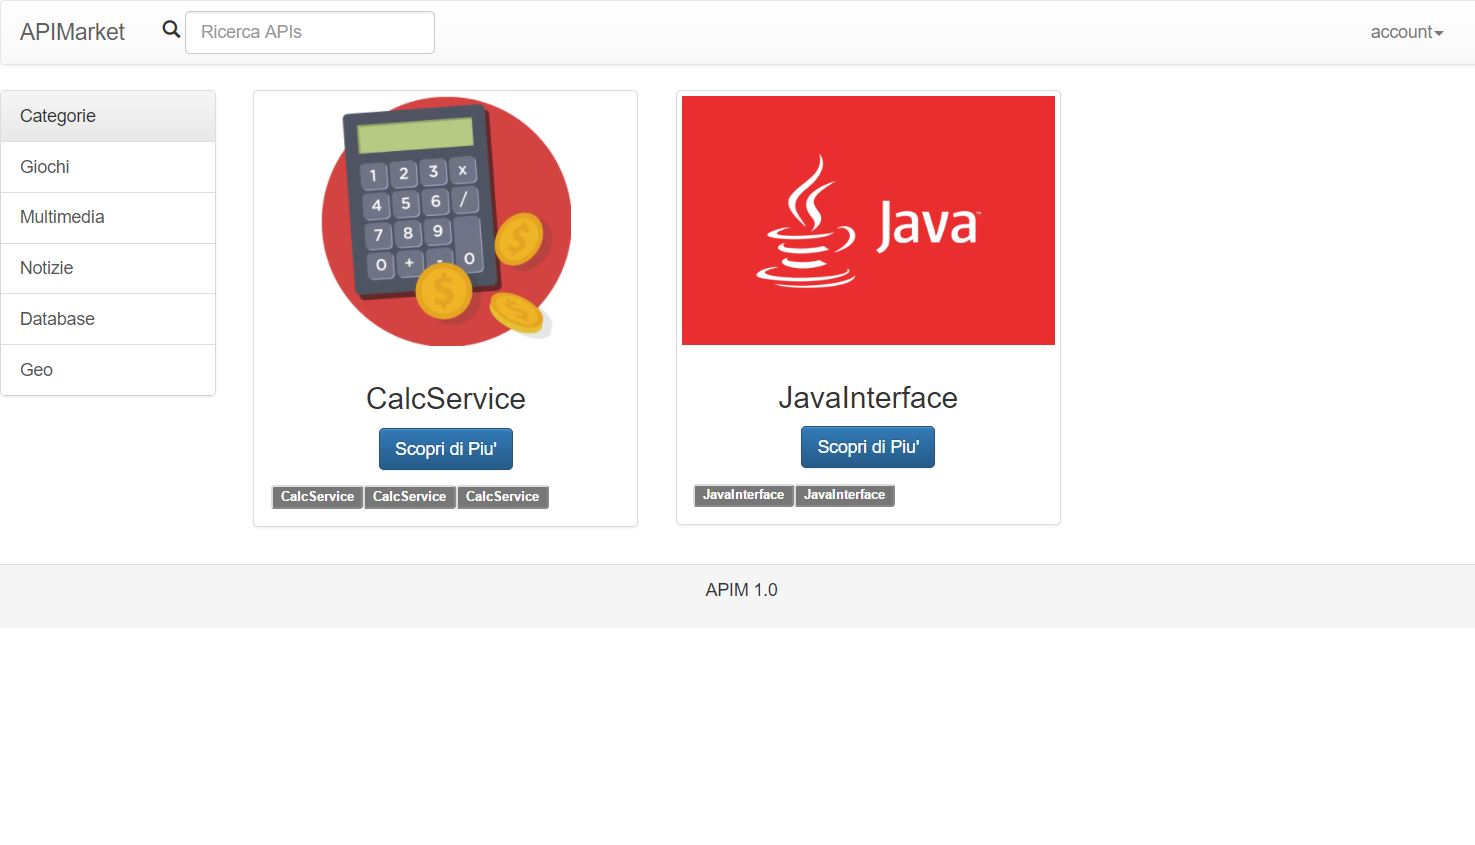
\includegraphics[scale=0.29]{img/APIM_home.JPG}}
			\caption{Homepage}
		\end{figure}
		
		Dalla schermata principale sono possibili le principali funzionalità dell'utente non autenticato. L'utente può registrarsi e autenticarsi tramite il menu in alto a destra, mentre a sinistra può sfogliare le varie categorie di API esposte nel market. Tramite la barra di ricerca, posta alla destra del logo del market, può effettuare una ricerca tramite keyword. Nella parte centrale dell'immagine sono disponibili le ultime otto API inserite all'interno dell'API Market.
		In fondo alla pagina è presente il footer, che contiene alcune informazioni sull'API Market.
		Come è possibile notare nella Figura 1, per la homepage, come per il resto della piattaforma è stato scelto un layout minimale e semplice per renderlo di facile utilizzo a diverse tipologie di utente.

	\subsection{Registrazione}
	Per poter usufruire delle funzionalità complete dell'API Market, quali acquisto e vendita di API, è necessario registrarsi. \MakeUppercase{è} possibile registrarsi alla piattaforma premendo il pulsante preposto nella barra superiore. La schermata che apparirà all'utente sarà la seguente:
	
	\label{Registrazione}
	\begin{figure}[H]
		\centering
		\fbox{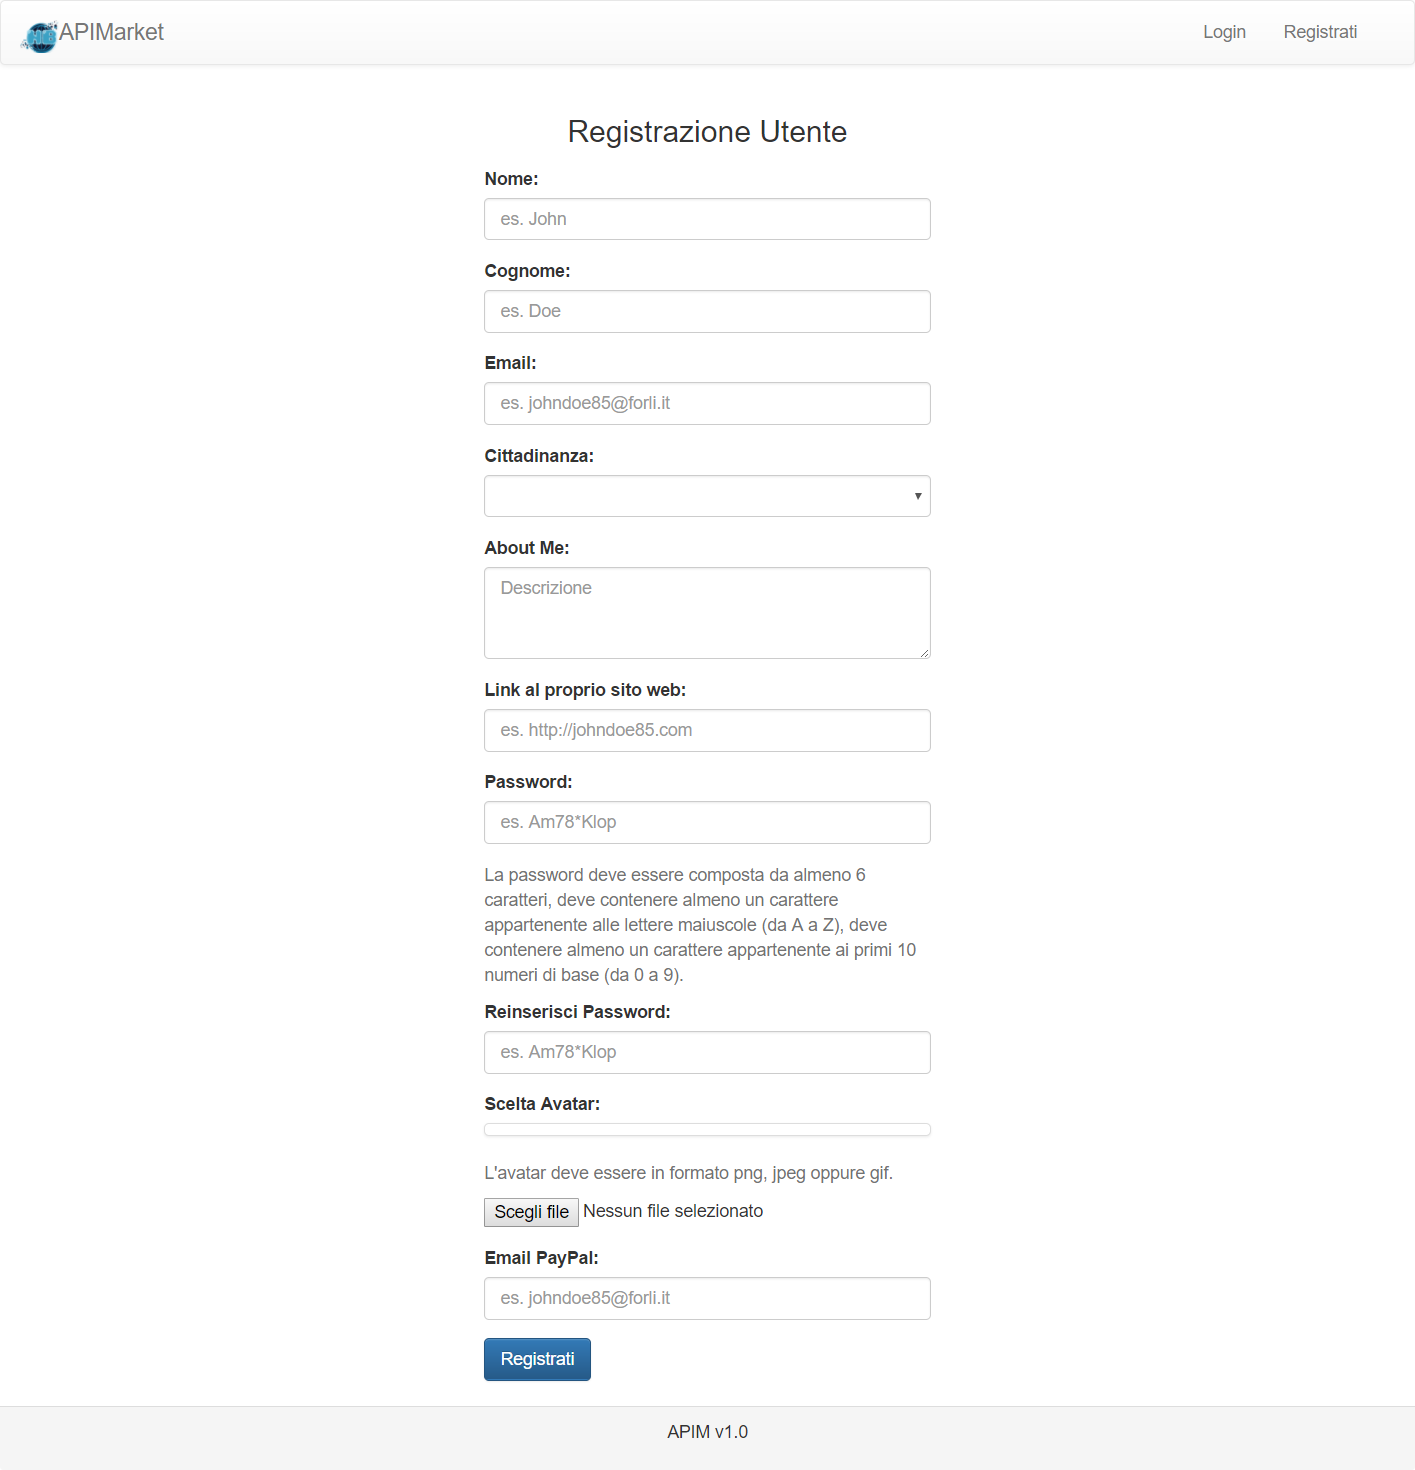
\includegraphics[scale=0.31]{img/APIM_registrazione.JPG}}
		\caption{Registrazione}
	\end{figure}
	
	Un utente per registrarsi dovrà compilare correttamente i seguenti campi, che sono obbligatori:
	\begin{itemize}
		\item Nome;
		\item Cognome;
		\item Username desiderato;
		\item Stato di residenza;
		\item Indirizzo e-mail;
		\item Password desiderata;
		\item Conferma password.
	\end{itemize}
	
	Qualora questi dati non fossero presenti o corretti, il sistema segnala un errore all'atto di registrazione e l'utente deve inserire dei parametri validi nei campi indicati. Sono presenti inoltre dei campi opzionali, destinati all'utente che vuole essere anche sviluppatore:
	
	\begin{itemize}
		\item Descrizione personale;
		\item Immagine personale;
		\item Email PayPal.
	\end{itemize}
	
	Questi campi, seppur non obbligatori, bloccano la registrazione qualora il loro inserimento non fosse effettuato in modo corretto. Si prega di prestare attenzione ai requisiti visualizzati nella schermata di registrazione.
	
	\subsection{Login}
	
	Tramite la barra superiore, vicino al pulsante di registrazione è possibile effettuare il login. La schermata di login può essere visualizzata a partire da ogni pagina non autenticata, selezionando l'apposita voce.
	Il login può essere effettuato da un utente precedentemente registrato e dalla schermata di login è possibile autenticarsi nella piattaforma per poter svolgere le funzionalità preposte agli utenti registrati. 
	
	\label{Login}
	\begin{figure}[H]
		\centering
		\fbox{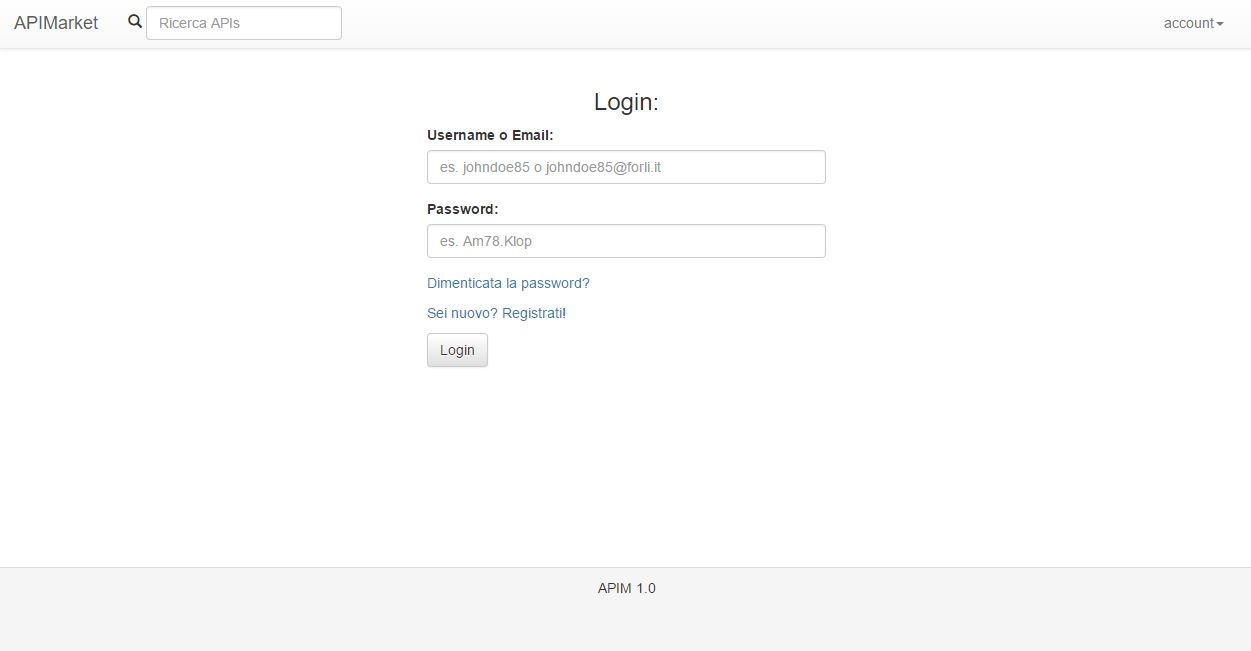
\includegraphics[scale=0.31]{img/APIM_login.JPG}}
		\caption{Login}
	\end{figure}
	
	\subsection{Conferma Login}
	Dopo aver inserito i dati di login e cliccato sul pulsante "Login", se i dati di accesso sono corretti, l'utente visualizza una pagina di conferma login, con la possibilità di recarsi sulla Homepage oppure nella gestione del proprio profilo.
	
	\label{Conferma Login}
	\begin{figure}[H]
		\centering
		\fbox{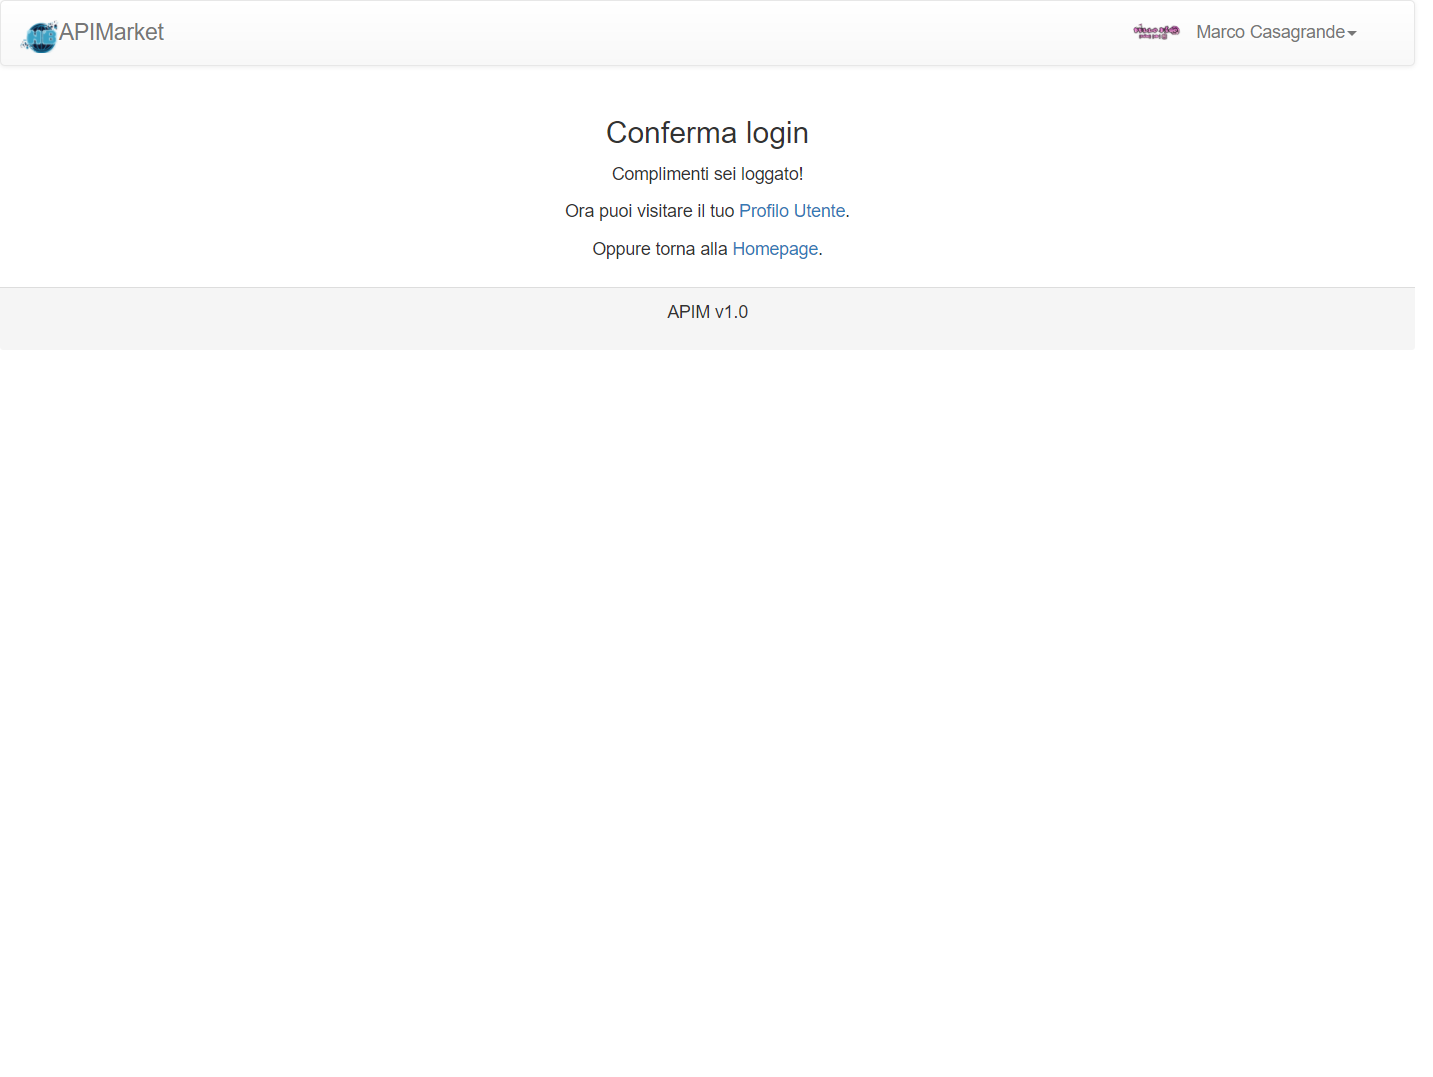
\includegraphics[scale=0.31]{img/APIM_confermaLogin.jpg}}
		\caption{Login}
	\end{figure}
	
	
	
	\subsection{Recupero Password}
	Qualora si fosse dimenticata la password, dalla schermata di login si può accedere alla pagina per il recupero della password. Inserendo l'indirizzo email si può ottenere un link per reimpostare i propri dati personali tramite una pagina dedicata. 
	
	\label{Recupero Password}
	\begin{figure}[H]
		\centering
		\fbox{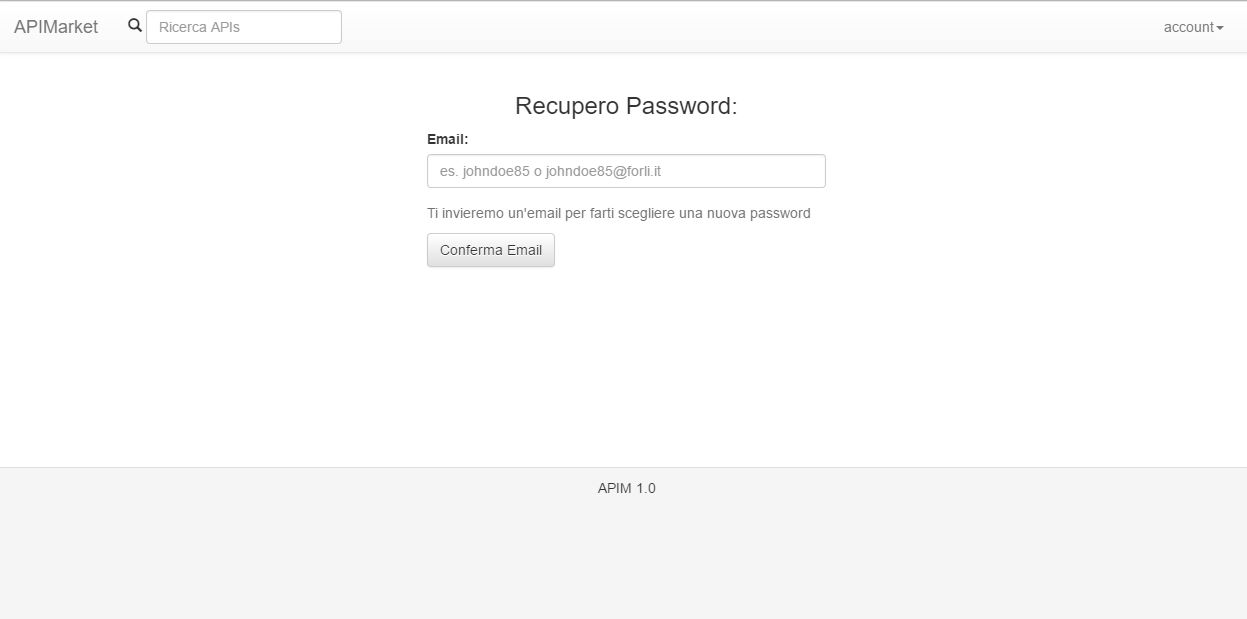
\includegraphics[scale=0.31]{img/APIM_recuperoPSW.JPG}}
		\caption{Recupero Password}
	\end{figure}

\subsection{Ricerca e visualizzazione API}

\subsubsection{Ricerca}
La funzionalità di ricerca è disponibile per qualsiasi categoria di utente. Essa permette, in base ad una parola chiave, di visualizzare le API relative contenute nella piattaforma. In seguito a ricerca, effettuata scrivendo sull'apposita barra la parola chiave desiderata, si può accedere ad un elenco dei risultati come mostrato. 

\label{Risultati ricerca}
\begin{figure}[H]
	\centering
	\fbox{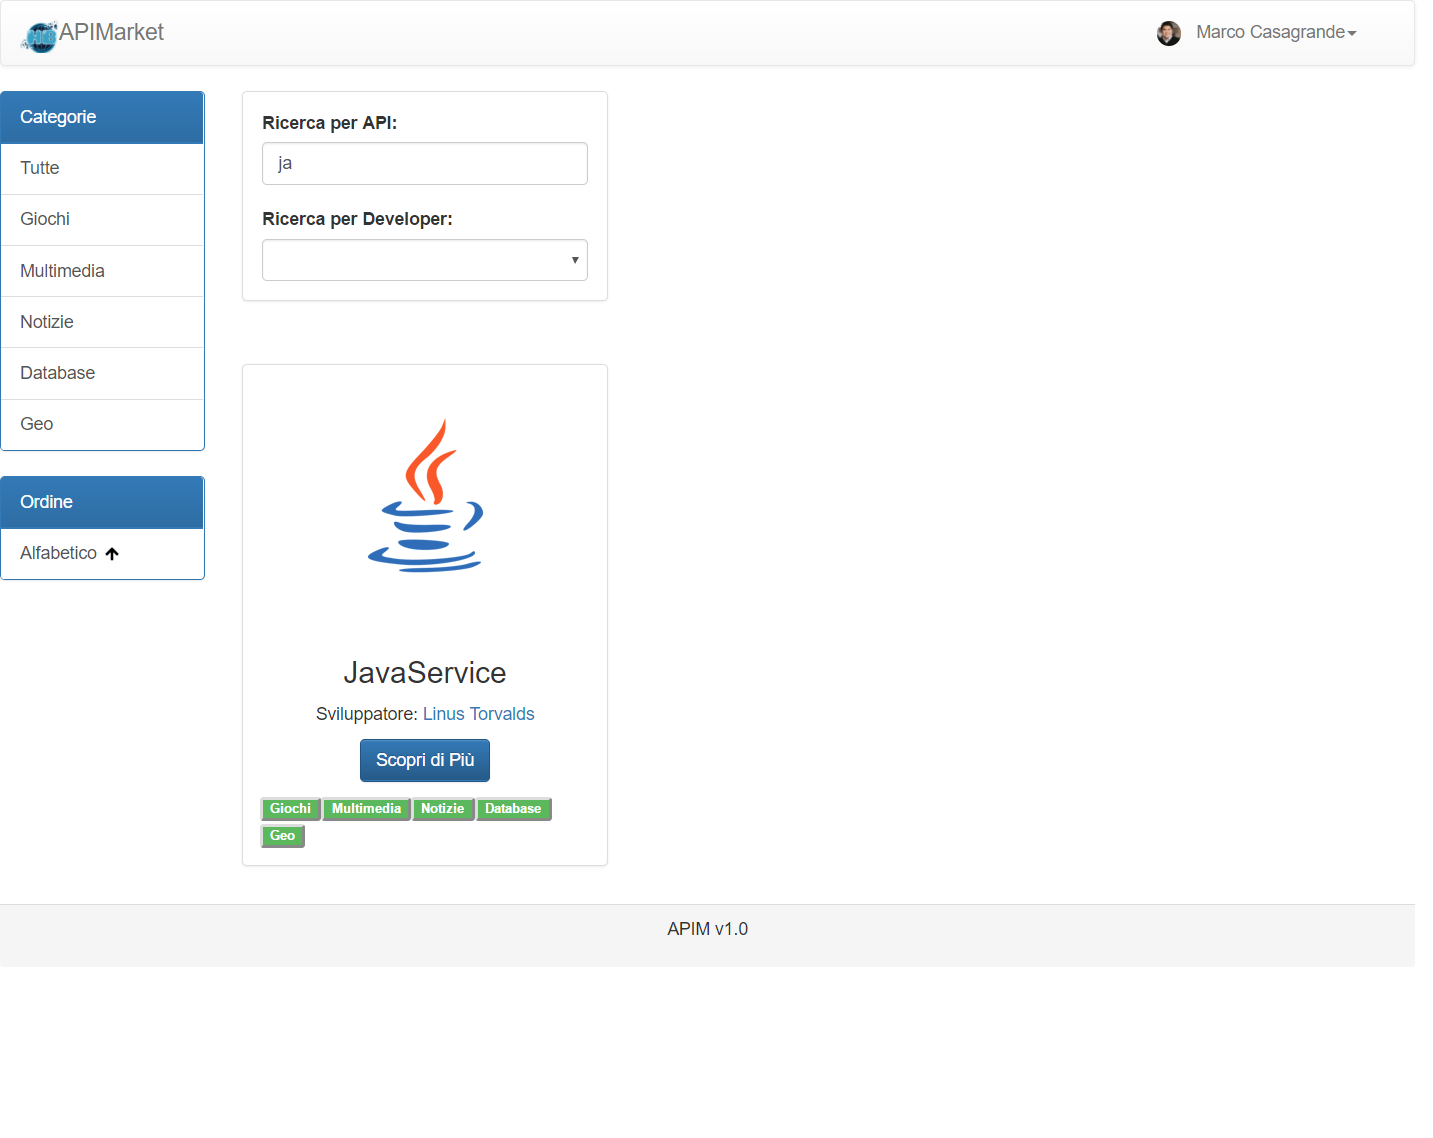
\includegraphics[scale=0.31]{img/APIM_ricerca.JPG}}
	\caption{Risultati ricerca}
\end{figure}


\subsubsection{Visualizzazione dettagli API}
Selezionando un API dall'elenco dei risultati, è possibile visualizzare i dati nel dettaglio, con relative specifiche. 


\label{Visualizzazione API}
\begin{figure}[H]
	\centering
	\fbox{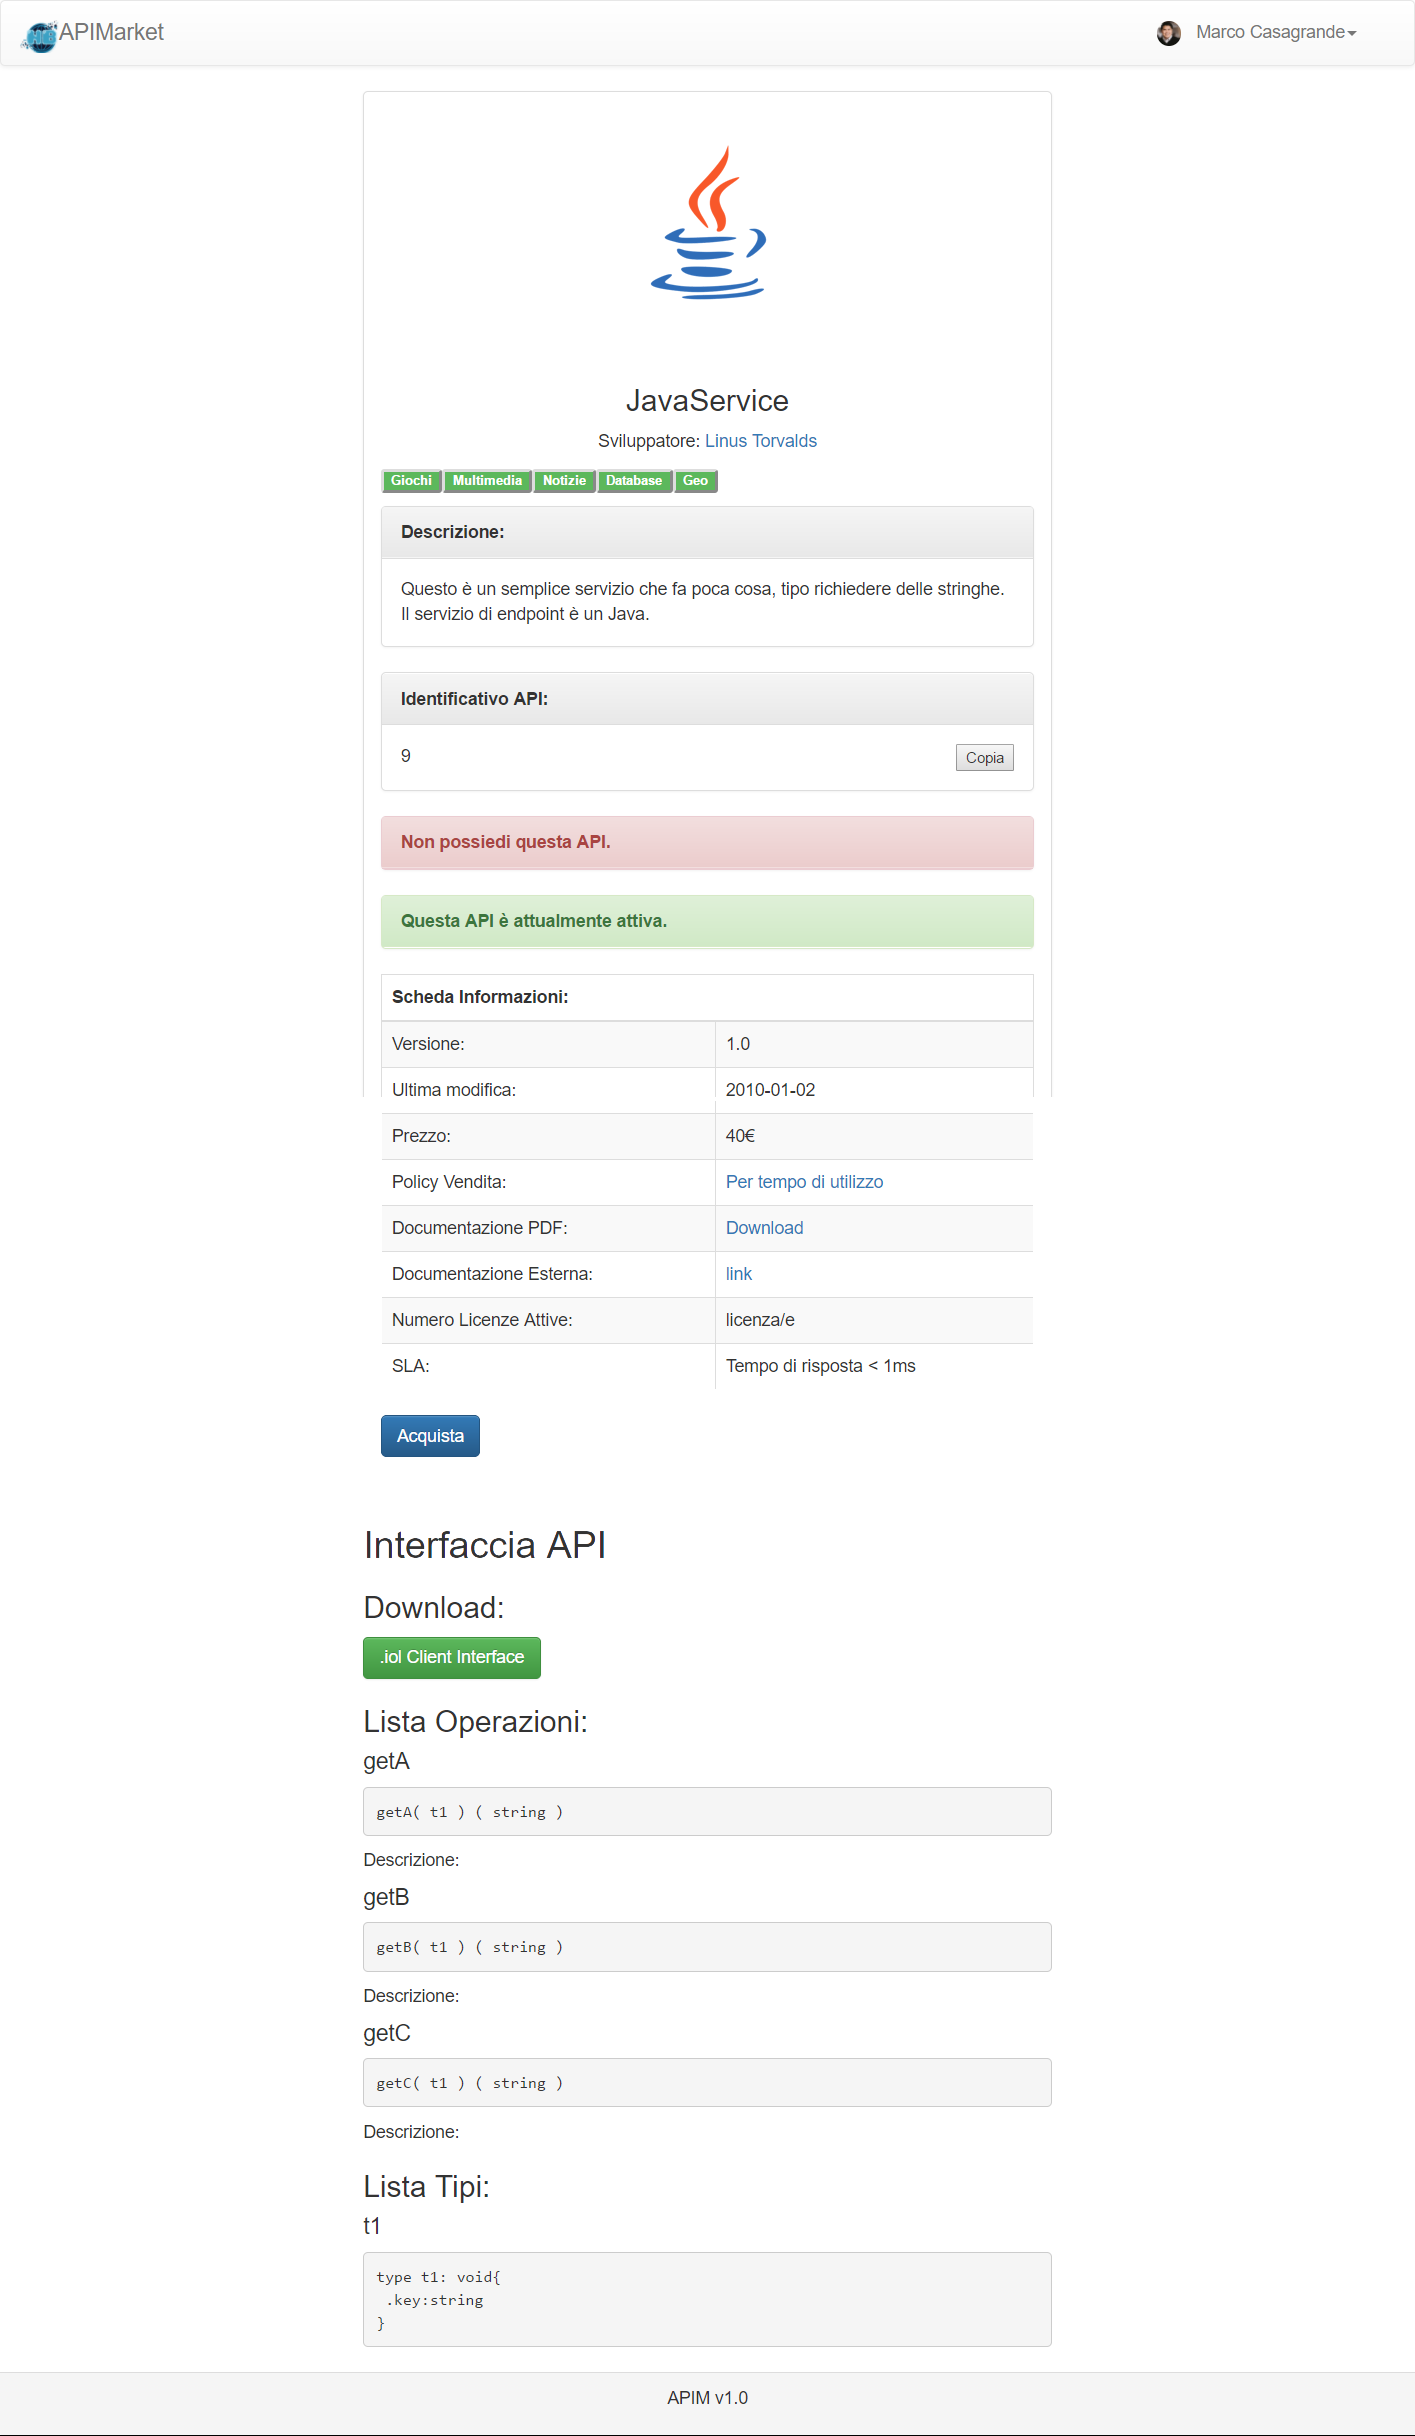
\includegraphics[scale=0.28]{img/APIM_dettagliApi.png}}
	\caption{Visualizzazione API}
\end{figure}

Ciascuna API presente nella piattaforma è caratterizzata da una policy di vendita, descritta all'interno di ciascun prodotto. E' possibile visualizzare i dettagli della policy clickando sull'apposito link nella schermata.

\label{Visualizza policy API}
\begin{figure}[H]
	\centering
	\fbox{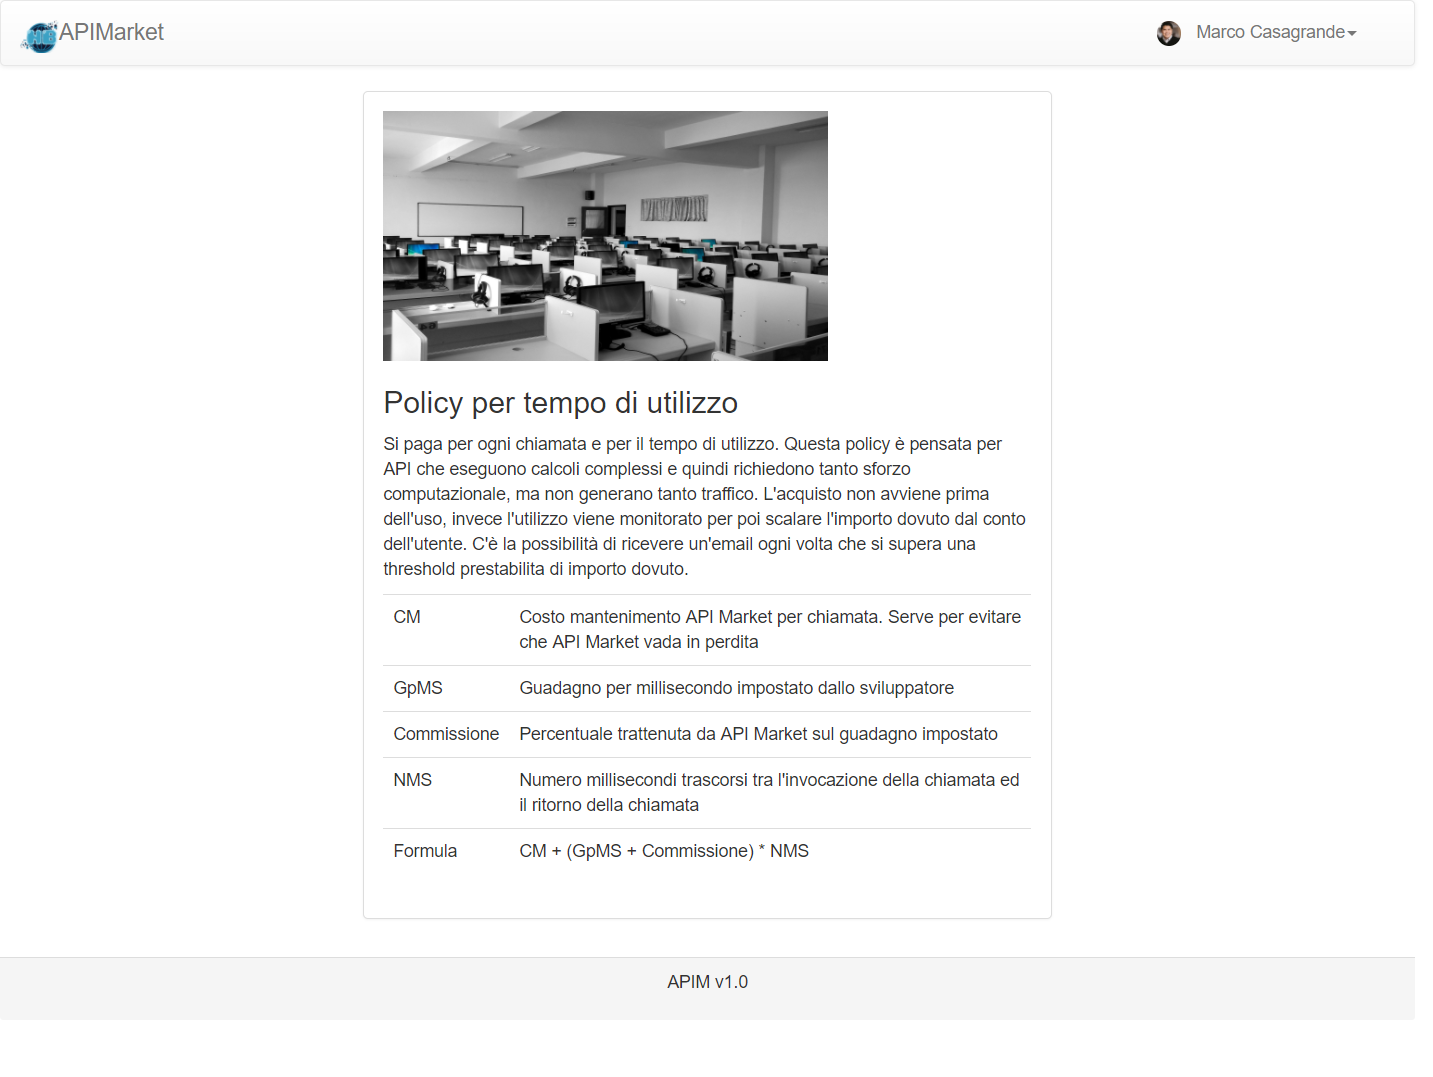
\includegraphics[scale=0.31]{img/APIM_policy.JPG}}
	\caption{Visualizza policy API}
\end{figure}

\subsubsection{Acquisto}
Qualora si decidesse di effettuare l'acquisto, nella schermata è presente un pulsante Acquista. Nella stessa schermata un utente loggato può inserire la quantità che intende acquistare, altrimenti chiederà di effettuare il login o la registrazione. Per maggiori relativi all'acquisto, si rimanda alla sezione 4.2 del presente manuale.





\newpage
\section{Cliente}

\subsection{Gestione profilo}

Una volta effettuato con successo il login, è possibile accedere al proprio profilo utente. La schermata principale relativa al profilo apparirà come nella figura sottostante.

\label{Profilo utente}
\begin{figure}[H]
	\centering
	\fbox{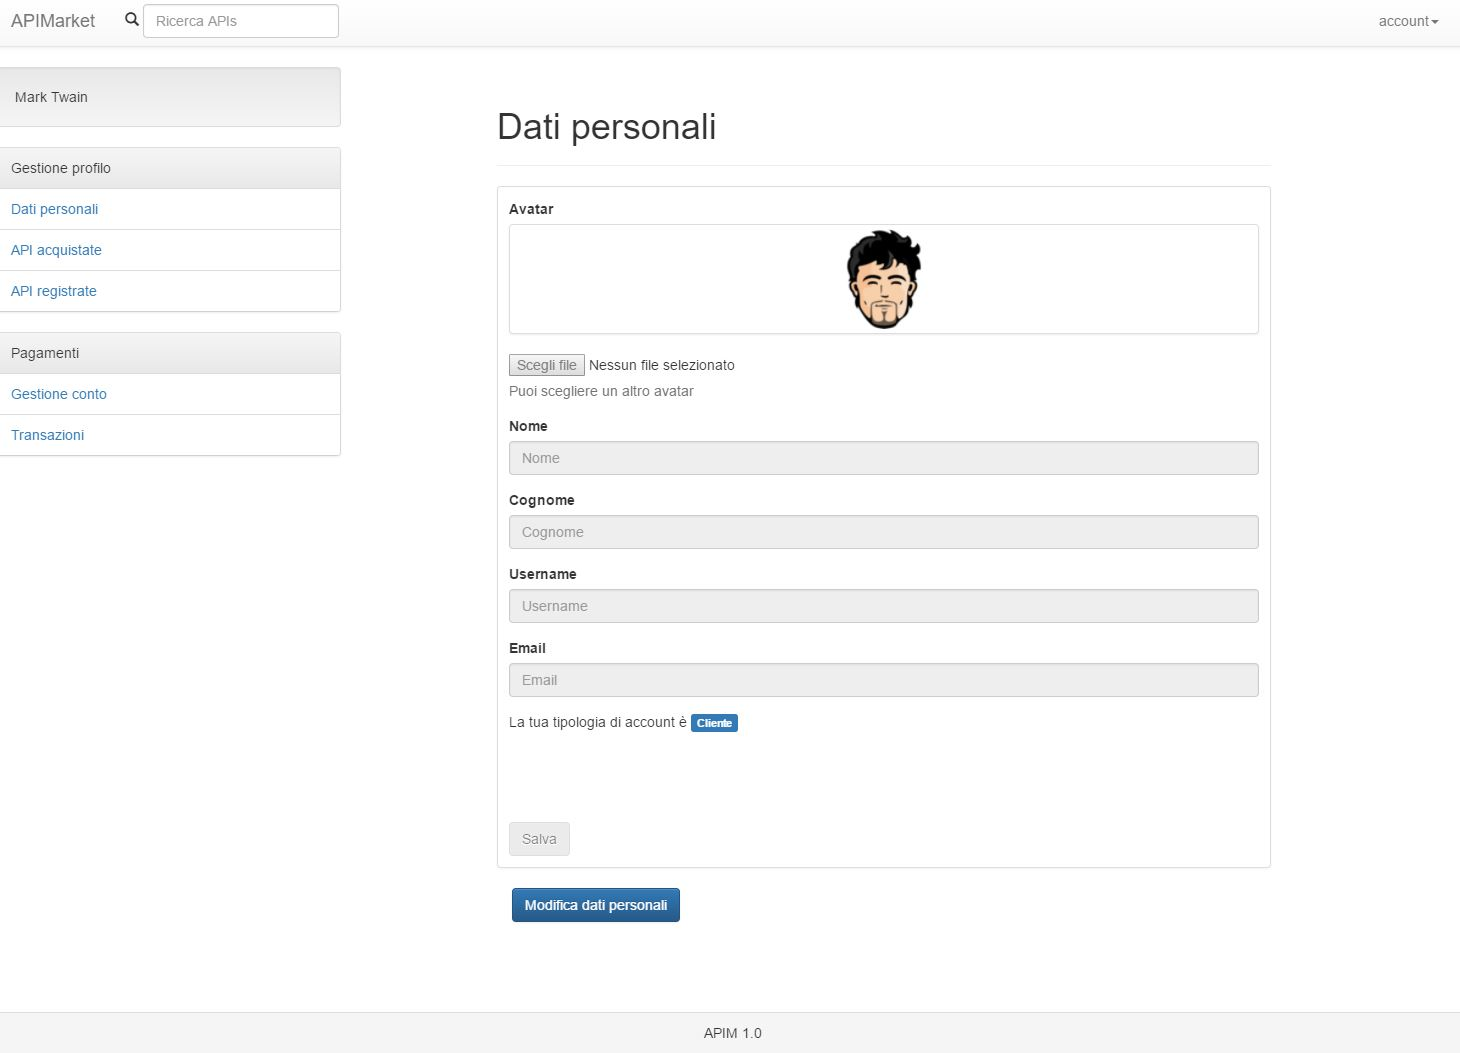
\includegraphics[scale=0.31]{img/APIM_account.JPG}}
	\caption{Profilo utente}
\end{figure}

Dalla schermata si potranno modificare i dati personali, inseriti al momento della registrazione, quali la propria anagrafica o dati relativi all'account quali l'immagine personale. E' visualizzato inoltre a quale gruppo di utenza si appartiene: l'utente registrato semplice infatti è un utente denominato "cliente", mentre l'utente abilitato al caricamento e alla vendita di servizi è denominato utente "Developer".

Tramite il menù laterale è possibile navigare nelle schermate del proprio profilo. Clickando sulla voce API acquistate si potrà consultare l'elenco delle api attualmente in possesso o acquistate in passato con i relativi dati. 

\label{API acquistate}
\begin{figure}[H]
	\centering
	\fbox{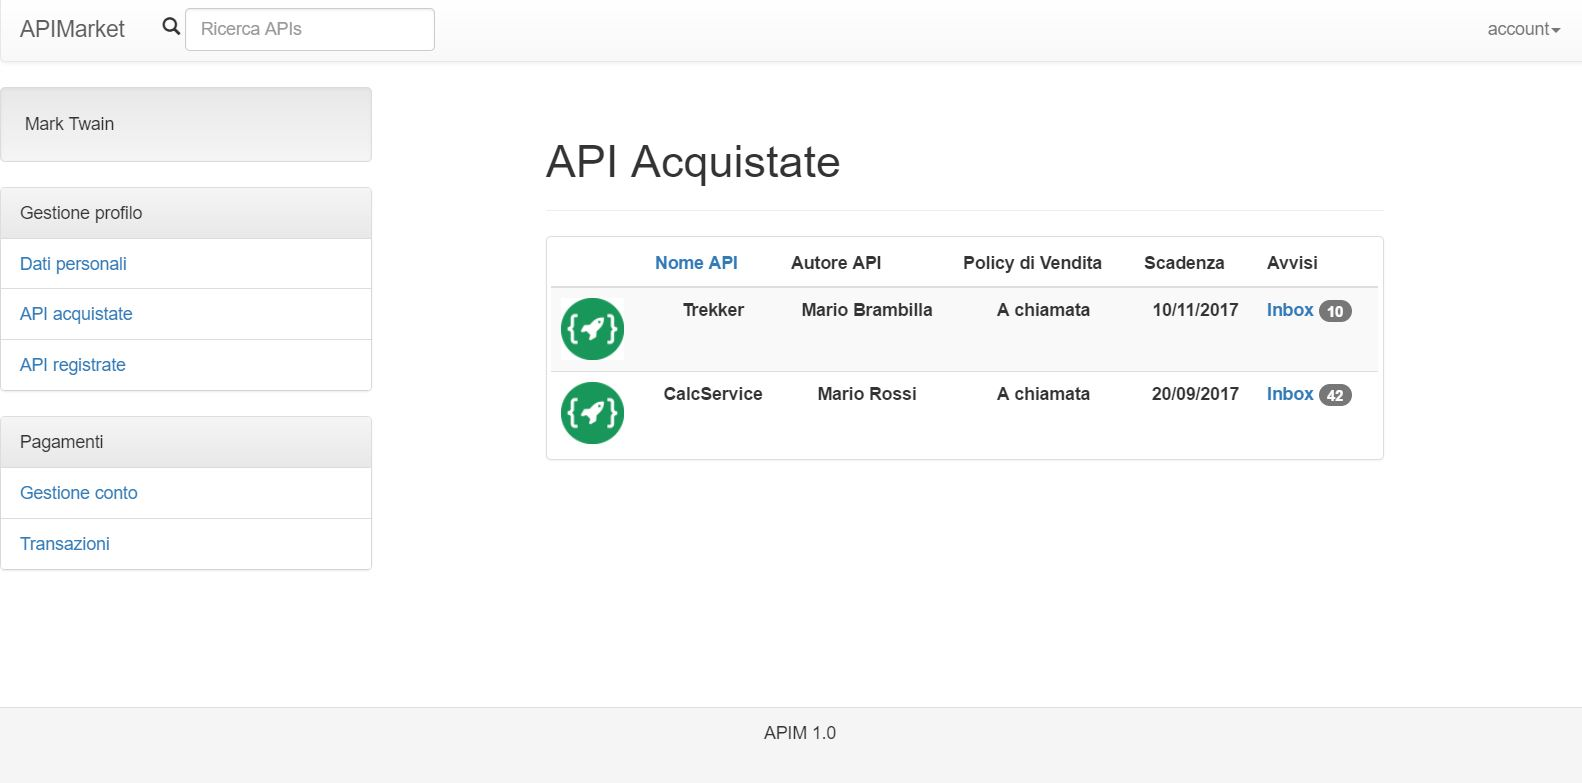
\includegraphics[scale=0.31]{img/APIM_apiAcquistate.JPG}}
	\caption{API acquistate}
\end{figure}
Nell'elenco delle API Acquistate è possibile rinnovare un'API prossima alla scadenza tramite l'apposito pulsante. L'utente effettuerà così una nuova transazione.


\subsection{Acquisto API}
Un cliente può acquistare una API direttamente dalla pagina di dettaglio API tramite il pulsante Acquista. 

All'interno della pagina relativa al completamento della transizione, l'utente potrà scegliere l'importo da acquistare a seconda della policy dell'API che intende acquistare.  

Una volta completata la transazione l'utente riceverà un API key con la quale potrà utilizzare il servizio acquistato. 

\label{Acquisto API}
\begin{figure}[H]
	\centering
	\fbox{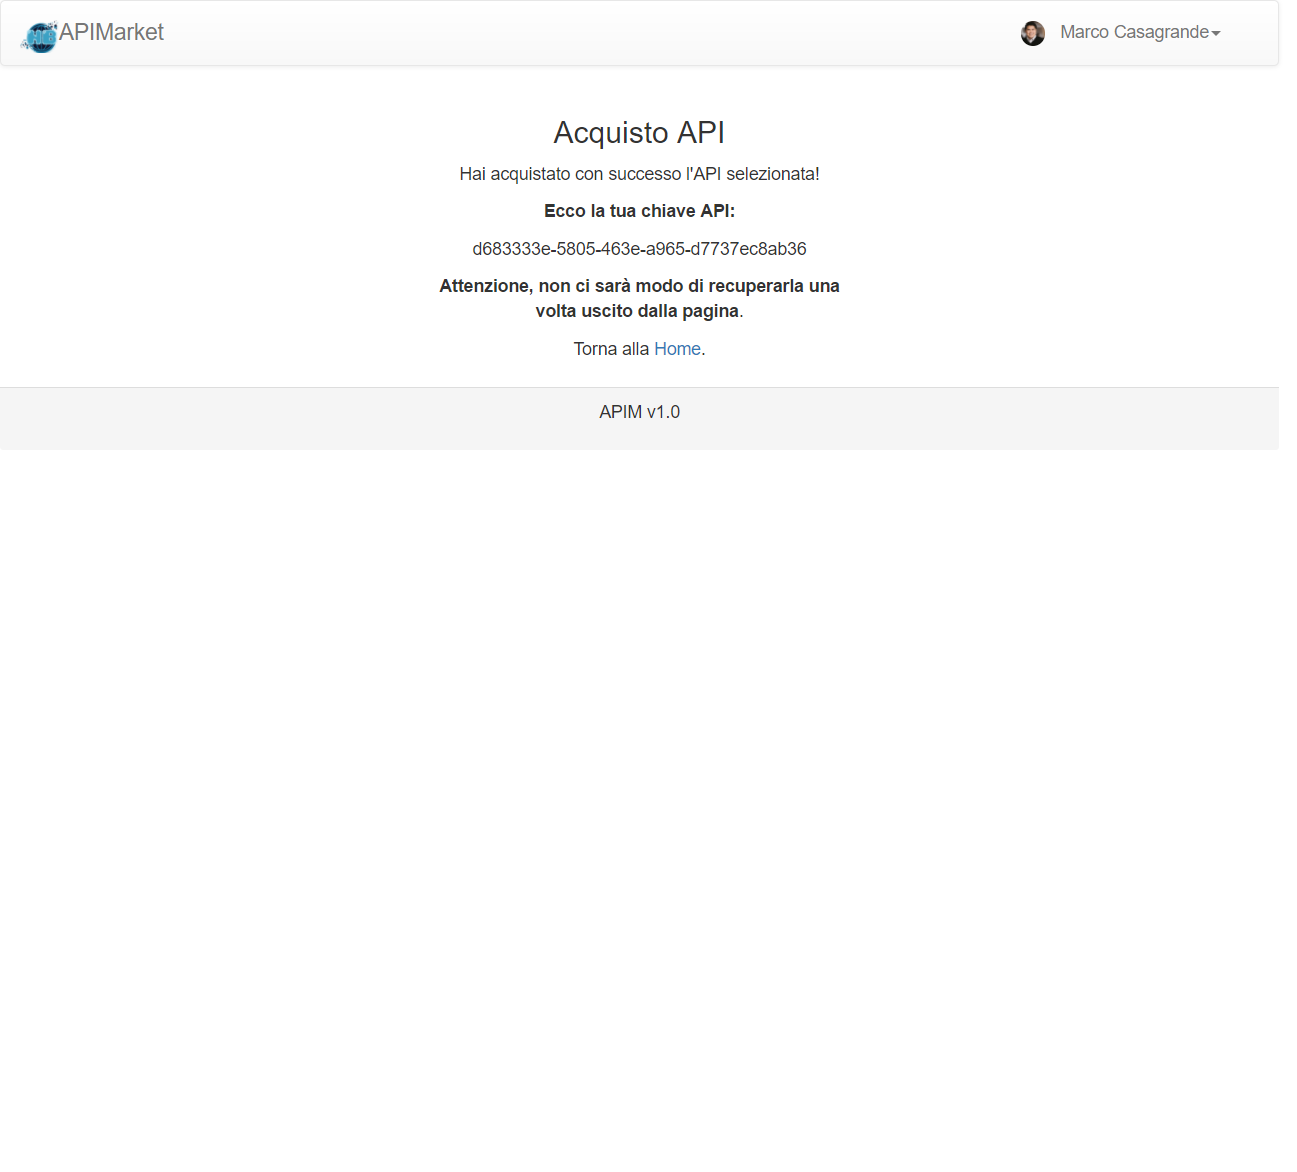
\includegraphics[scale=0.31]{img/APIM_confermaAcquisto.png}}
	\caption{Acquisto API}
\end{figure}

\subsection{Acquisto crediti}
Dalla gestione del profilo, un utente è in grado di acquistare crediti utilizzabili per pagare le API. Un utente può acquistare un numero di crediti a scelta tra i tagli presenti nell'apposita pagina. Nella pagina successiva l'utente completa la transazione e il saldo crediti del suo conto viene aggiornato con i nuovi crediti sommati ai precedenti.

\label{Acquisto Crediti}
\begin{figure}[H]
	\centering
	\fbox{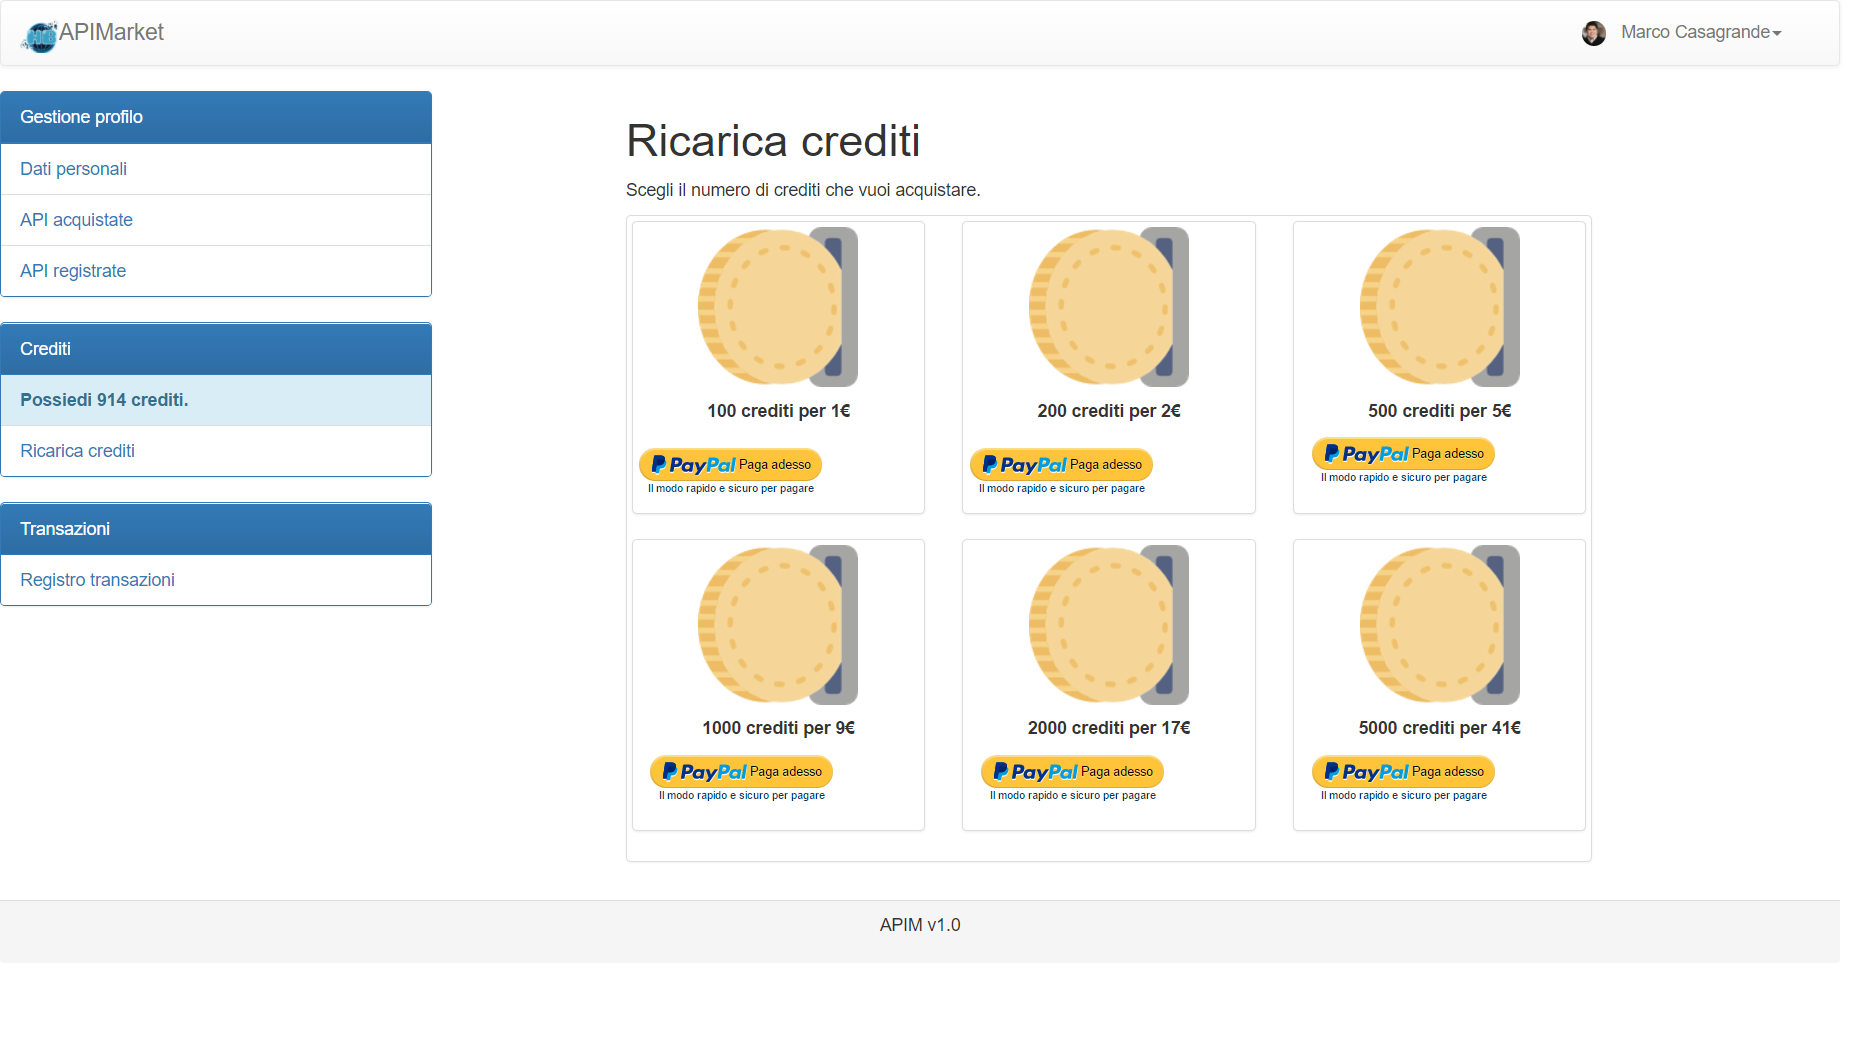
\includegraphics[scale=0.31]{img/APIM_acquistoCrediti.JPG}}
	\caption{Acquisto Crediti}
\end{figure}


\newpage
\section{Sviluppatore}
Lo sviluppatore è in grado di eseguire tutte le operazioni disponibili al cliente e in aggiunta può inserire API nel market e trasferire il guadagno proveniente dalla vendita nel suo saldo Paypal.
Uno sviluppatore deve inserire, se non fatto al momento della registrazione i seguenti dati obbligatori:
	
\begin{itemize}
	\item Descrizione personale;
	\item Immagine personale;
	\item Email PayPal.
\end{itemize}


\subsection{API registrate}
Lo sviluppatore all'interno della sua area personale può visualizzare le API registrate e le loro caratteristiche principali.

\label{API registrate}
\begin{figure}[H]
	\centering
	\fbox{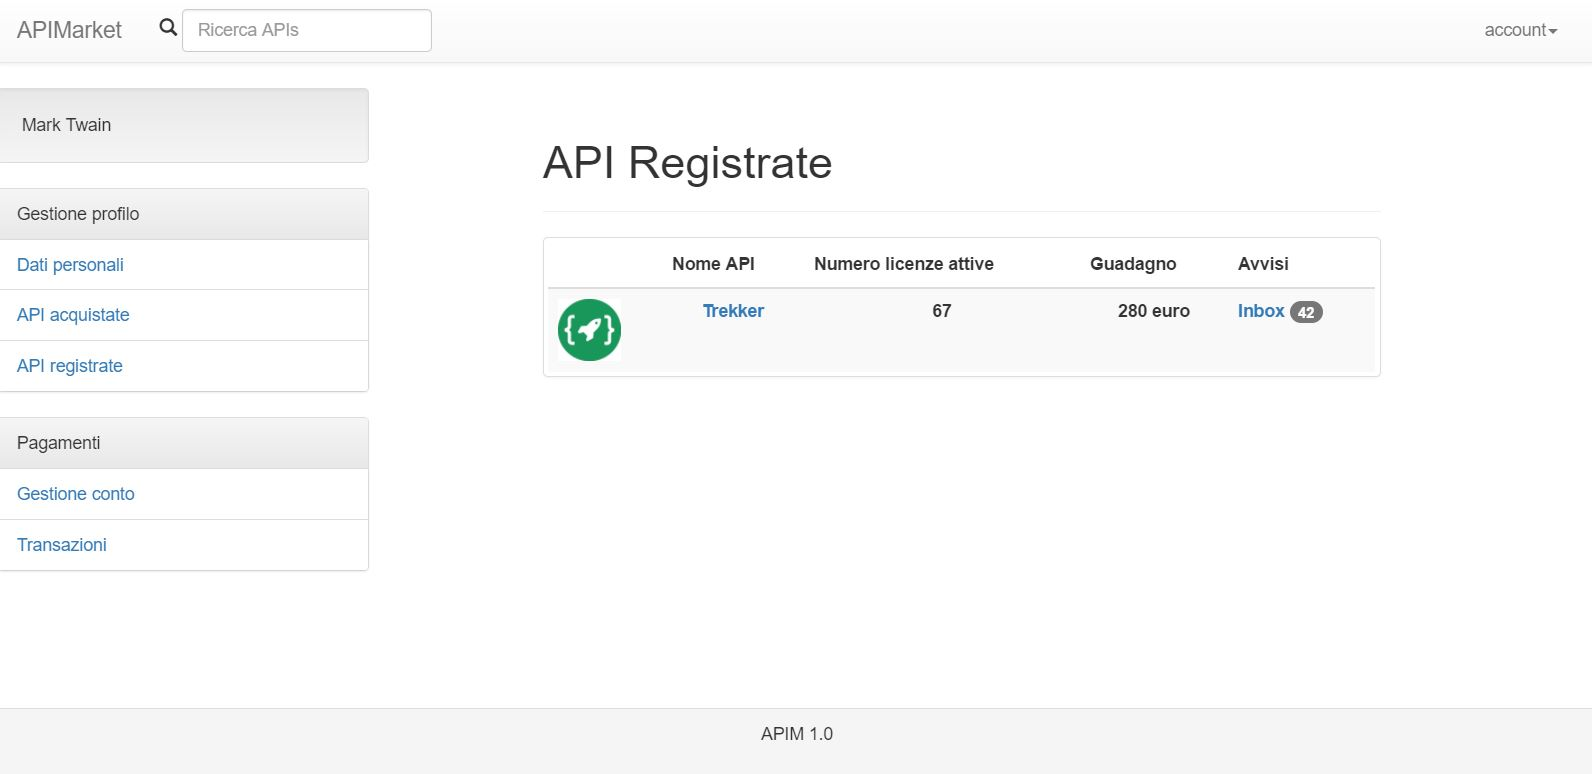
\includegraphics[scale=0.31]{img/APIM_apiRegistrate.JPG}}
	\caption{API registrate}
\end{figure}

\subsection{Registrazione API}

L'utente abilitato alla vendita (Sviluppatore) può  registrare le proprie API per la vendita nell'apposita pagina accessibile dal profilo utente. La schermata per la registrazione di nuove API appare come mostrato nell'immagine sottostante.

\label{Registrazione API}
\begin{figure}[H]
	\centering
	\fbox{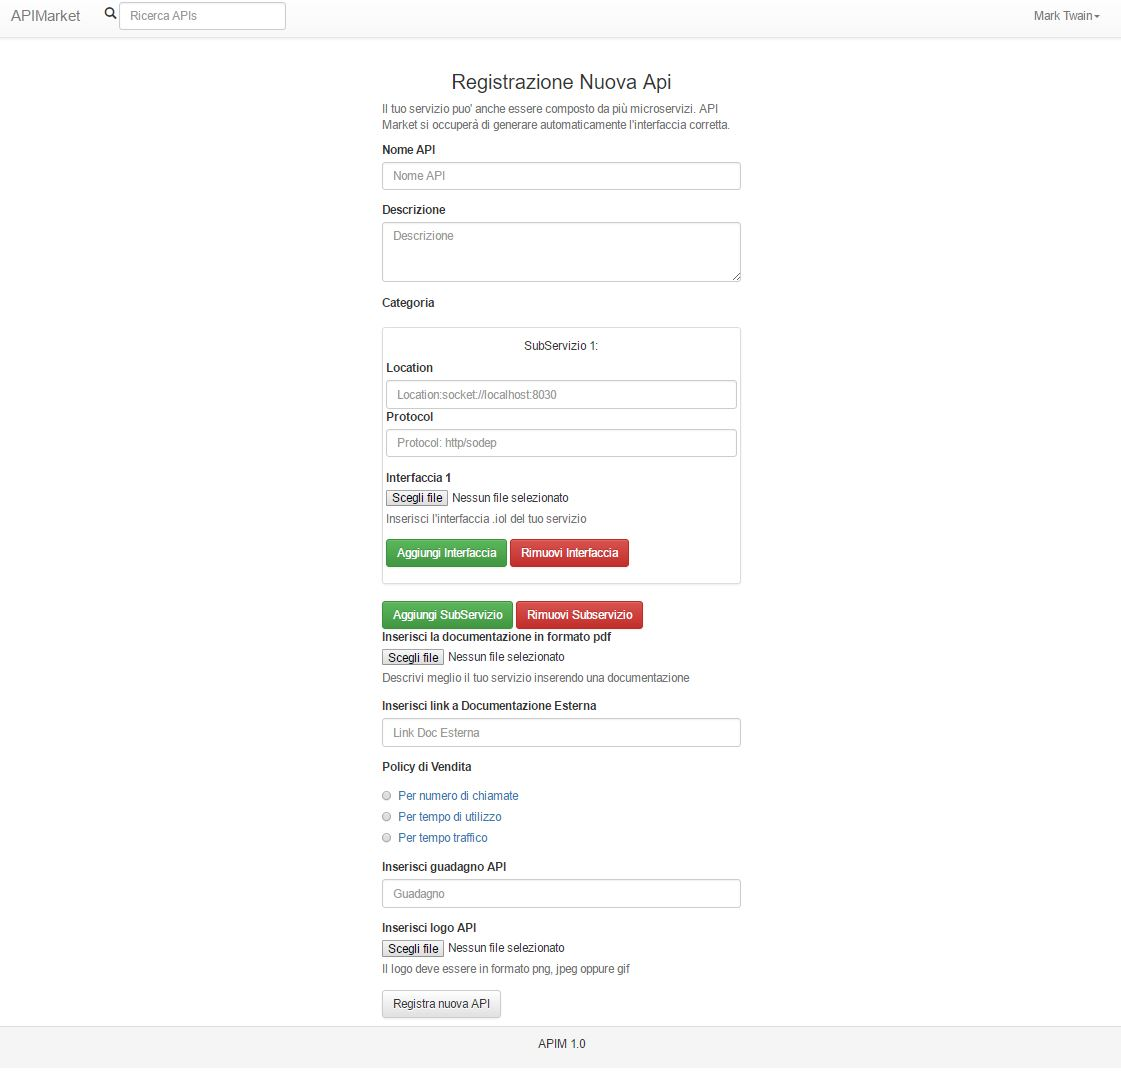
\includegraphics[scale=0.31]{img/APIM_nuovaApi.JPG}}
	\caption{Registrazione API}
\end{figure}

All'interno, l'utente dovrà specificare obbligatoriamente i seguenti dati per permettere l'inserimento del proprio prodotto nella piattaforma

\begin{itemize}
	\item Nome dell'API;
	\item Breve descrizione;
	\item Tags che identificano le categorie a cui appartiene;
	\item L'URI/Posizione del servizio;
	\item Il protocollo di comunicazione utilizzato;
	\item I file che caratterizzano l'interfaccia;
	\item Posizione, protocollo e interfaccia di eventuali sottoservizi correlati (opzionale);
	\item Documentazione PDF o link esterno;
	\item Il guadagno desiderato e la policy scelta;
	\item Il logo del prodotto.
\end{itemize}

Qualora i campi inseriti fossero corretti, il sistema segnala che la procedura è andata a buon fine.

\subsection{Pagamenti}
Lo sviluppatore accumula il guadagno della vendita delle sue API, nel suo conto personale; esso può decidere di trasferire il ricavato sul suo conto Paypal, collegato all'indirizzo email inserito nel suo profilo.
L'operazione è possibile tramite il pulsante "NOME PULSANTE" per poi completare la transazione sul sito PAYPAL???

IMMAGINE CONTO PERSONALE

\newpage
\section{Amministratore}
	\subsection{Login admin}
	Il login admin viene effettuato su una pagina speculare al login dell'utente ma in una pagina diversa; l'utente amministratore dovrà aggiungere \url{/logi_admin} all'indirizzo del marketplate \progetto.
	\label{Login amministratore}
	\begin{figure}[H]
		\centering
		\fbox{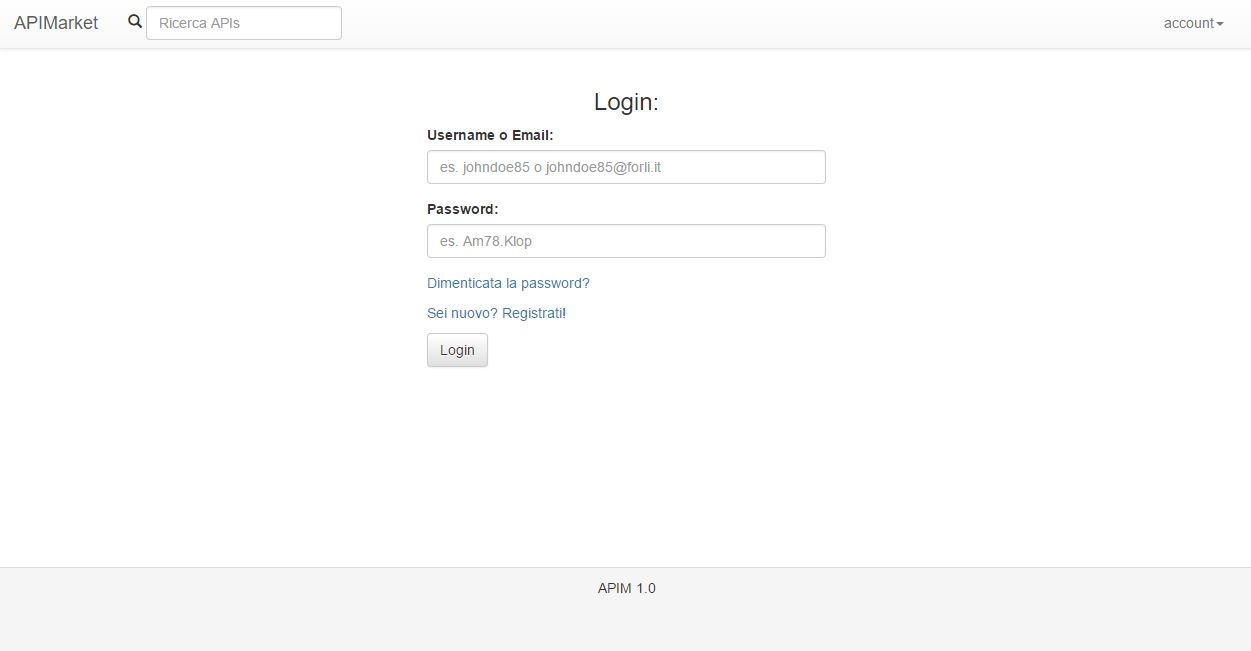
\includegraphics[scale=0.31]{img/APIM_login.JPG}}
		\caption{Login amministratore}
	\end{figure}

\subsection{Pannello amministratore}
	L'ammistratore entrerà in un pannello, dove sulla sinistra può scegliere cose moderare.
	
		\label{Pannello amministratore}
	\begin{figure}[H]
		\centering
		\fbox{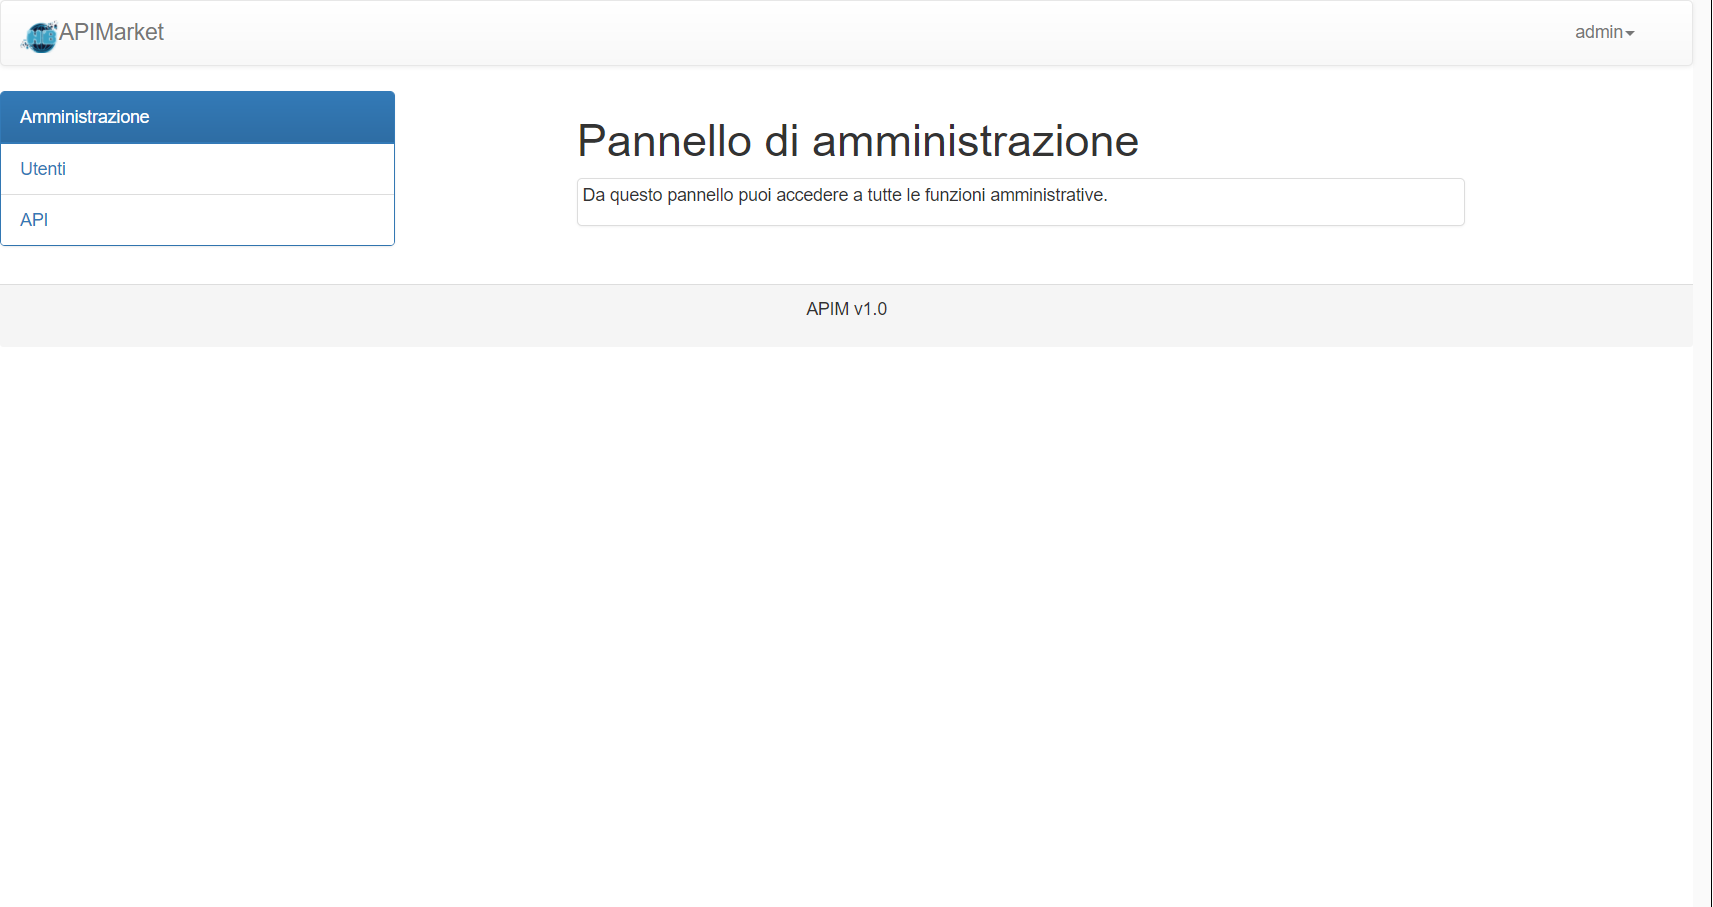
\includegraphics[scale=0.31]{img/APIM_pannelloAdmin.png}}
		\caption{Pannello amministratore}
	\end{figure}
	
	
\subsection{Moderazione API}
Selezionando la voce API, l'amministratore potrà intervenire su tutte le API presenti sul market. Le operazioni possibili sono la sospensione, attivazione e cancellazione di una API, come mostrato di seguito.

	\label{Moderazione API}
	\begin{figure}[H]
		\centering
		\fbox{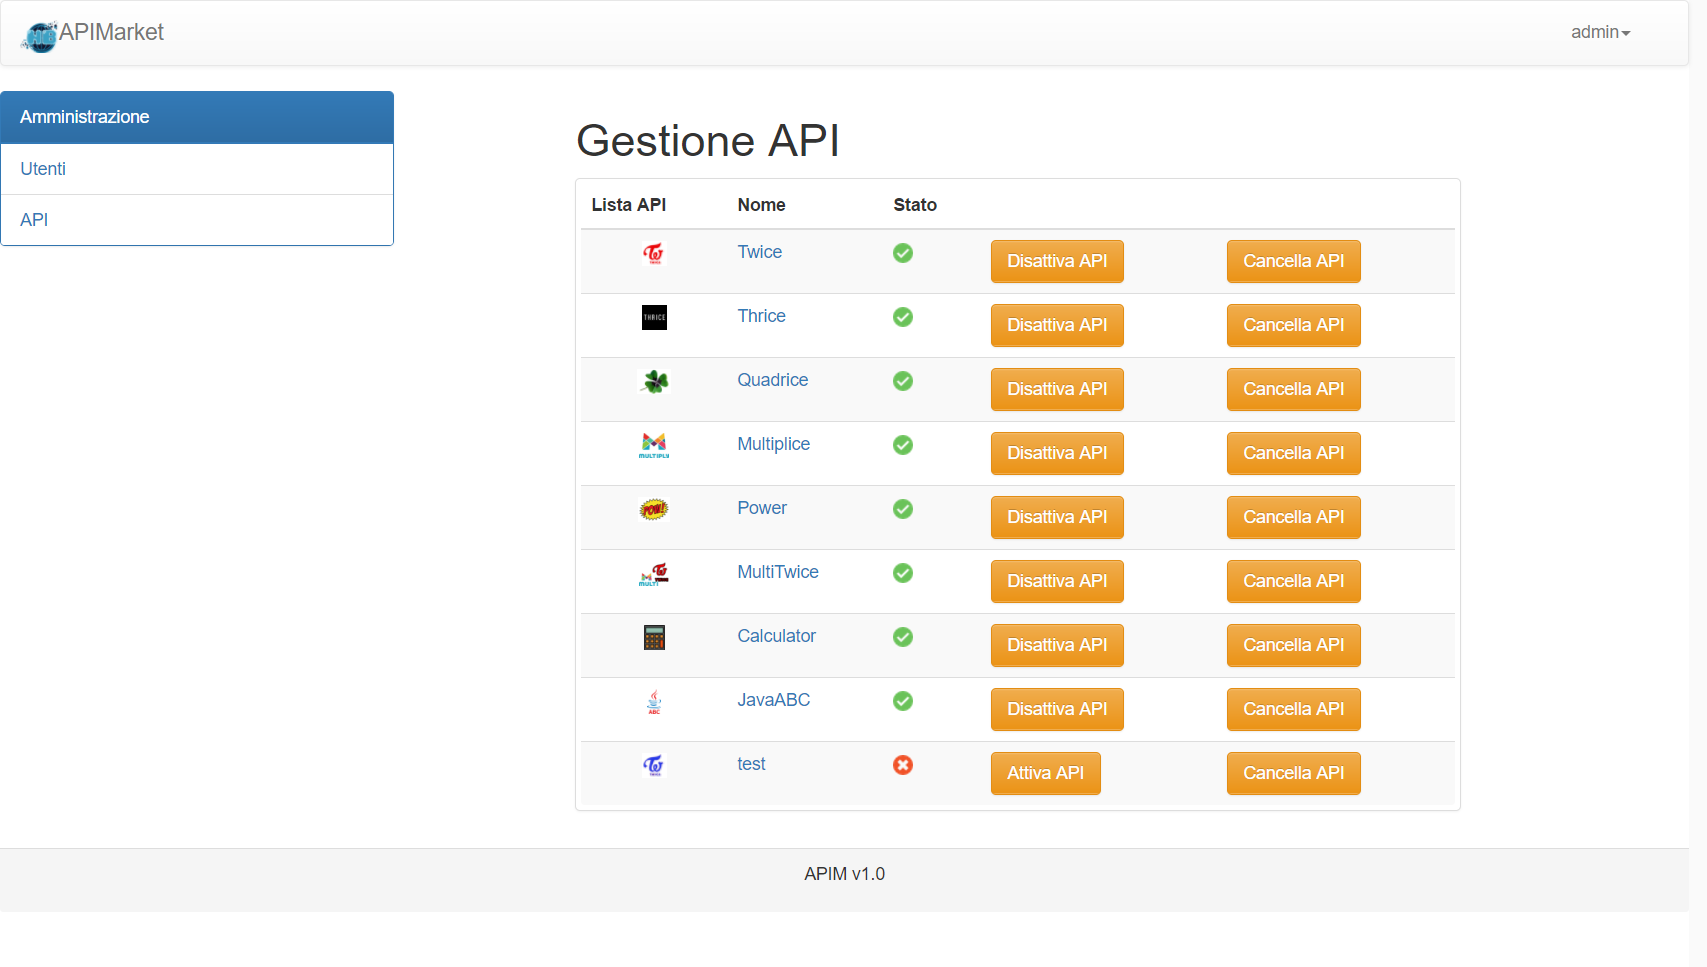
\includegraphics[scale=0.31]{img/APIM_modificaAPI.png}}
		\caption{Moderazione API}
	\end{figure}


\subsection{Moderazione Utente}
Selezionando la voce Utenti, l'amministratore potrà visualizzare le API registrate e attive di tutti gli utenti, con la possibilità di eliminare gli utenti, come mostrato nella seguente immagine.

\label{Moderazione Utente}
\begin{figure}[H]
	\centering
	\fbox{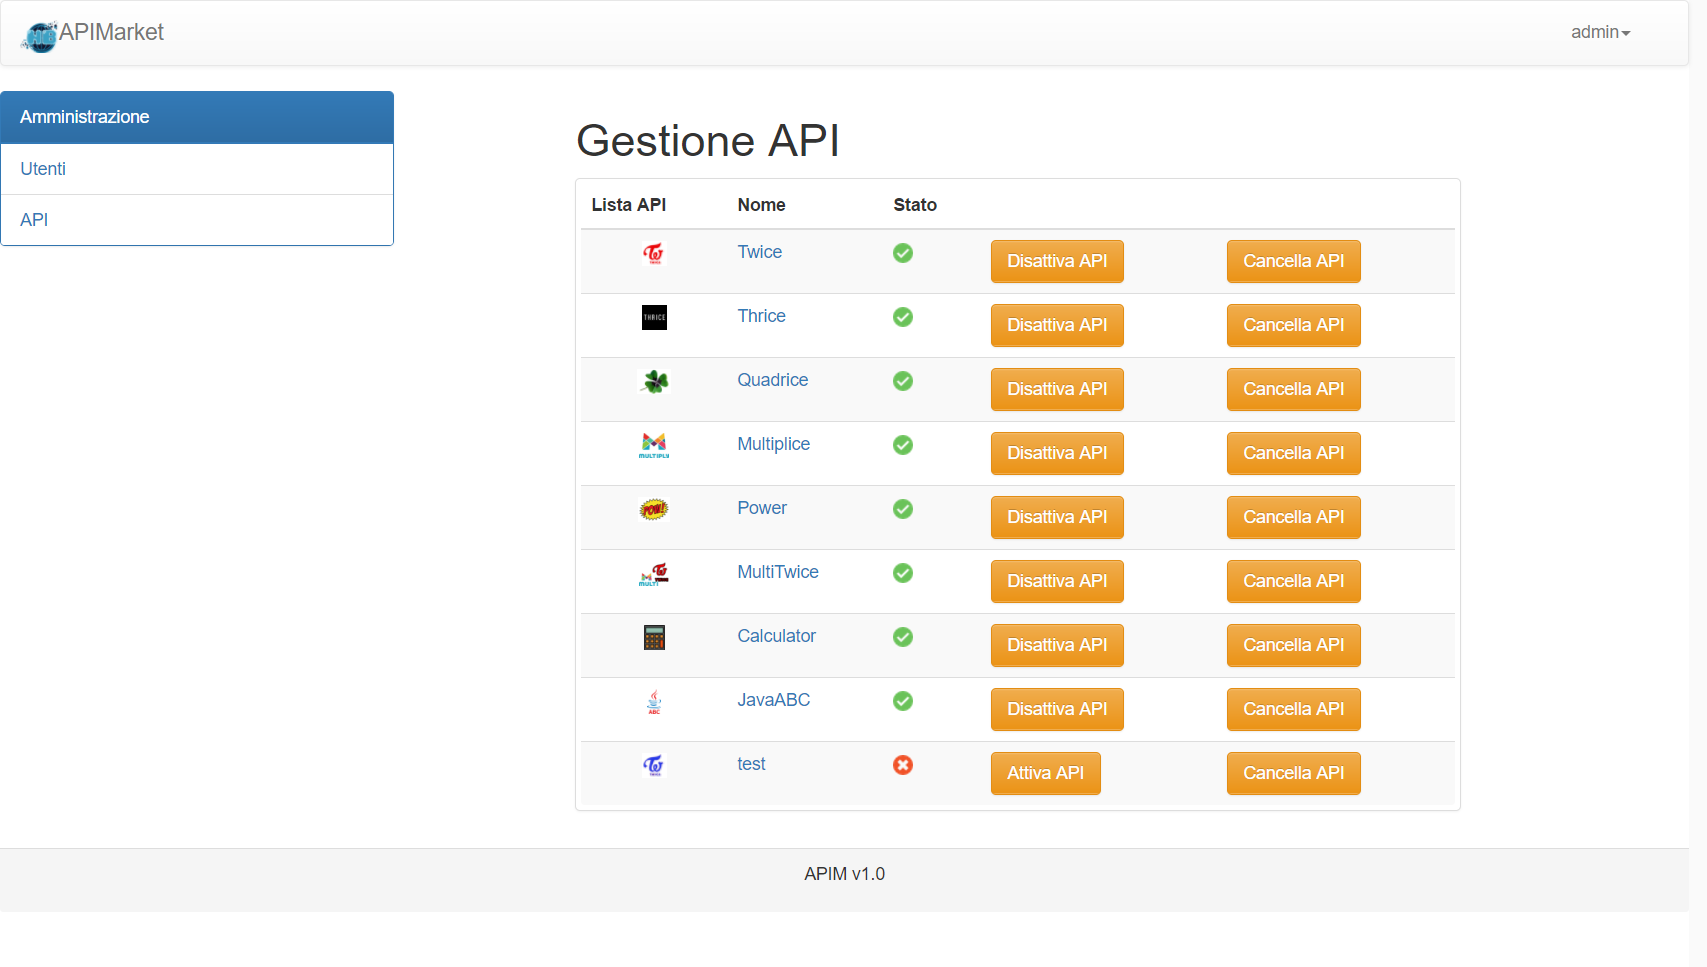
\includegraphics[scale=0.31]{img/APIM_modificaAPI.png}}
	\caption{Moderazione Utente}
\end{figure}

\newpage
\section{Segnalazione degli errori}


L'utente ha la possibilità di segnalare eventuali errori e malfunzionamenti del servizio API Market, descrivendo il problema trovato nella apposita sezione Issue all'interno del profilo GitHub del gruppo Netbreak (\url{https://github.com/netbreakswe/APIM_Source/issues}).

\appendix
\newpage
\section{Glossario}

%\hypertarget{A}{}

\newglossaryentry{AlexaSDK}
{
	name=AlexaSDK,
	description={sistema di comando vocale sviluppato da Amazon}
}
\newglossaryentry{Android}
{
	name=Android,
	description={sistema operativo open source per dispositivi mobili, sviluppato da Google Inc. e basato su kernel Linux. Inoltre, mette a disposizione una piattaforma per lo sviluppo di applicazioni per dispositivi mobili}
}
\newglossaryentry{Angular2}
{
	name=Angular 2,
	description={framework gratuito per il front-end web, open source ed evoluzione di AngularJS. \MakeUppercase{è} scritto in linguaggio TypeScript}
}
\newglossaryentry{API}
{
	name=API,
	description={acronimo per Application Programming Interface, indica un insieme di funzioni software ad alto livello disponibili al programmatore. Solitamente sono composte di poche istruzioni volte alla realizzazione di una specifica azione. Un esempio di API sono le librerie software messe a disposizione da un certo linguaggio di programmazione}
}
\newglossaryentry{API Gateway}
{
	name=API Gateway,
	description={strumento che filtra e reindirizza le richieste utente per le varie API, fornendo il servizio, anche se questo non è presente sul server del marketplace}
}
\newglossaryentry{API Key}
{
	name=API Key,
	description={codice che identifica univocamente una specifica API e funge da token segreto che ne regola l'accesso e l'utilizzo}
}
\newglossaryentry{API Market}
{
	name=API Market,
	description={piattaforma che permette il commercio di API}
}
\newglossaryentry{Asana}
{
	name=Asana,
	description={applicazione web, disponibile anche per dispositivi mobili, progettata per aiutare i team di progetto a monitorare il proprio lavoro e migliorare la collaborazione. Ogni progetto è composto di più attività, chiamate task, le quali richiedono lo svolgimento di determinati compiti. Gli utenti possono aggiungere note, commenti, allegati e tag, il tutto notificando, via email automatica o notifica push, ogni altro membro del team che lavora al progetto}
}
\newglossaryentry{Astah}
{
	name=Astah,
	description={strumento di modellazione UML per la creazione di vari tipi di diagrammi. La versione Community è gratuita, a differenza di quella Professional}
}
\newglossaryentry{AWS}
{
	name=AWS,
	description={acronimo per Amazon Web Services, rappresenta una collezione di servizi di cloud computing che compongono la piattaforma on demand (su richiesta) offerta dall'azienda Amazon. Questi servizi sono operativi in 12 regioni geografiche in cui Amazon stessa ha suddiviso il globo. Tra questi servizi i più conosciuti sono Amazon Elastic Compute Cloud (EC2) e Amazon Simple Storage Service (S3)}
}
\newglossaryentry{AWS Lambda}
{
	name=AWS Lambda,
	description={servizio di elaborazione serverless, che esegue il codice utente in risposta a determinati eventi e gestisce automaticamente le risorse di elaborazione, tra cui la manutenzione di server e del sistema operativo, il provisioning e il ridimensionamento automatico della capacità, lo sviluppo di patch per codice e protezione e il monitoraggio e la creazione di log. Può essere usato per estendere altri servizi AWS con logica personalizzata oppure creare servizi di back-end in grado di operare con la scalabilità, le prestazioni e la sicurezza di AWS}
}


%\newpage
%\hypertarget{B}{}

\newglossaryentry{back-end}
{
	name=back-end,
	description={Parte di un sistema informatico che elabora i dati generati dal front-end}
}

\newglossaryentry{Bootstrap 3}
{
	name=Bootstrap 3,
	description={Framework gratuito per il front-end web, open source, per la progettazione di siti e applicazioni web. Contiene template CSS per la maggior parte delle componenti grafiche di un'interfaccia utente ed estensioni JavaScript. A differenza di molti altri framework web, Bootstrap si occupa solo della parte front-end}
}

\newglossaryentry{browser}
{
	name=browser,
	description={Applicazione per il recupero, la presentazione e la navigazione di risorse sul web}
}
%\newpage
%\hypertarget{C}{}

\newglossaryentry{Camel Case}
{
	name=Camel Case,
	description={La Notazione a Cammello o in inglese Camel Case è la pratica nata durante gli anni settanta di scrivere parole composte o frasi unendo tutte le parole tra loro, ma lasciando le loro iniziali maiuscole}
}

\newglossaryentry{client}
{
	name=client,
	description={componente che accede ai servizi o alle risorse messe a disposizione da un server. Esso fa parte dell'architettura logica di rete client-server. Inoltre, il termine client indica anche il software usato sul computer-client per accedere alle funzionalità offerte da un server}
}

\newglossaryentry{cloud computing}
{
	name=cloud computing,
	description={letteralmente "nuvola informatica", indica un paradigma di erogazione di risorse informatiche come l'archiviazione, l'elaborazione o la trasmissione di dati, caratterizzato dalla disponibilità on demand attraverso Internet, a partire da un insieme di risorse preesistenti e configurabili}
}

\newglossaryentry{CSS}
{
	name=CSS,
	description={acronimo per Cascading Style Sheets (letteralmente fogli di stile a cascata), è un linguaggio usato per definire la formattazione di documenti HTML, XHTML e XML}
}

\newglossaryentry{CSS3}
{
	name=CSS3,
	description={ultima versione dello standard CSS. \MakeUppercase{è} retrocompatibile con le precedenti versioni di CSS}
}

\newglossaryentry{CSSLint}
{
	name=CSSLint,
	description={strumento che aiuta a rilevare possibili errori nel codice CSS}
}

\newglossaryentry{customer communication dashboard}
{
	name=customer communication dashboard,
	description={interfaccia grafica che organizza e presenta le informazioni circa l'acquisto o la disdetta di API in modo semplice, intuitivo ed immediato, consentendo al management di agire tempestivamente nella correzione della strategia in caso di necessità}
}



	

%\newpage
%\newpage
\section{D}

\begin{itemize}
	\item \textbf{Database NoSQL}: si differenziano dai database SQL per il fatto che i dati vengono conservati in documenti e non in tabelle. Le informazioni non sono distribuite in differenti strutture logiche, ma vengono aggregate per oggetto in documenti, la cui natura può essere di tipo Key-Value (che rappresenta la forma primitiva di database NoSQL) o Document Store, basati su semantica JSON. Ogni documento aggregato raccoglie tutti i dati associati a un’entità, in modo che qualsiasi applicazione possa trattare l’entità come oggetto e valutare in un sol colpo tutte le informazioni a essa correlate. In questo modo, si evitano anche i fardelli computazionali dovuti ai passaggi di aggregazione delle informazioni tipici del linguaggio SQL, in quanto tutti i dati necessari e corrispondenti a un medesimo oggetto sono già disponibili in un unico documento. L’assenza di tabelle permette ai database non relazionali di essere schemaless, ossia privi di un qualsiasi schema definito a priori, e questa caratteristica conferisce ai database NoSQL un altro vantaggio non trascurabile.
	\item \textbf{Database SQL}: sono basati sul modello relazionale (RDBMS) progettato per:
	\begin{enumerate}  
		\item Creare e modificare schemi di database (DDL - Data Definition Language);
		\item Inserire, modificare e gestire dati memorizzati (DML - Data Manipulation Language);
		\item Creare e gestire strumenti di controllo ed accesso ai dati (DCL - Data Control Language).
	\end{enumerate}
	\item \textbf{Diagramma dei package}: in UML, i packages vengono usati per raggruppare elementi e fornire un namespace per gli elementi raggruppati. Un package può contenere altri packages o altri elementi UML (ad esempio, classi, oggetti, casi d'uso, componenti, nodi, istanze di nodi, etc.), consentendo un'organizzazione gerarchica dei vari elementi che descrivono un sistema.
	\item \textbf{Diagramma delle classi}: tipo di diagramma che può comparire in un modello UML, il quale consente di descrivere tipi di entità, con le loro caratteristiche e le eventuali relazioni fra questi tipi. Gli strumenti concettuali utilizzati sono il concetto di classe del paradigma object-oriented e altri correlati, per esempio la generalizzazione, che è una relazione concettuale assimilabile al meccanismo object-oriented dell'ereditarietà
	\item \textbf{Diagramma di attività}: diagramma definito all'interno dello Unified Modeling Language (UML), che definisce le attività da svolgere per realizzare una data funzionalità. Può essere utilizzato durante la progettazione del software, per dettagliare un determinato algoritmo. In particolare, definisce le relazioni tra le attività, i responsabili per le singole attività e i punti di decisione. \MakeUppercase{è} spesso usato come modello complementare ai diagrammi dei casi d'uso, per descrivere le dinamiche con cui si sviluppano
	\item \textbf{Diagramma di Gantt}: è usato principalmente nelle attività di project management, ed è costruito partendo da un asse orizzontale, a rappresentazione dell'arco temporale totale del progetto, suddiviso in fasi incrementali, e da un asse verticale, a rappresentazione delle mansioni o attività che costituiscono il progetto. Un diagramma di Gantt permette la rappresentazione grafica di un calendario di attività, utile al fine di pianificare, coordinare e tracciare specifiche attività in un progetto, dando una chiara illustrazione dello stato d'avanzamento del progetto rappresentato.
	\item \textbf{Diagramma di sequenza}: diagramma previsto dallo standard UML, utilizzato per descrivere uno scenario, ovvero una sequenza di azioni in cui tutte le scelte sono state già effettuate. Descrive le relazioni che intercorrono, in termini di messaggi, tra attori, oggetti di business, oggetti o entità del sistema che si sta rappresentando
	\item \textbf{Django}: web framework open source per lo sviluppo di applicazioni web, scritto in linguaggio Python, seguendo il design pattern MVC (Model-View-Controller)
	\item \textbf{DynamoDB}: servizio di database NoSQL completamente gestito e messo a disposizione da Amazon. Esso consente di scaricare gli oneri amministrativi di funzionamento e di scalare un database distribuito, in modo che l'utente non debba preoccuparsi di nulla.
	Con DynamoDB, è possibile creare le tabelle del database in grado di memorizzare e recuperare qualsiasi quantità di dati, servire qualsiasi livello di richiesta di traffico, e utilizzare la console di gestione AWS per monitorare le metriche di utilizzo delle risorse e di prestazioni. Infine, diffonde automaticamente i dati e il traffico per le tabelle su di un numero sufficiente di server per gestire le esigenze dell'utente, mantenendo prestazioni costanti e veloci. Tutti i dati sono memorizzati su dischi SSD e replicati automaticamente su più Availability Zones (zone di disponibilità) in una regione AWS.
\end{itemize}



%\newpage
%\newpage
\section{E}

\begin{itemize}
	\item \textbf{ePub}: formato di file per e-book basato su XML, che possono essere scaricati e letti su dispositivi come smartphone, tablet, computer o e-reader. Il termine ePub viene spesso usato come abbreviazione di electronic publication.
	\item \textbf{Event-driven}: programmazione guidata dagli eventi o semplicemente, programmazione a eventi.
	\item \textbf{Express}: framework per Node.js per applicazioni web, rilasciato come software gratuito e open source sotto licenza MIT. È stato progettato per la creazione di applicazioni web e API. Express è utilizzato per la parte di back-end nello stack MEAN, assieme a MongoDB, come database, e AngularJS, per la parte di front-end.
\end{itemize}
	
%\newpage
%\newglossaryentry{Fagan Inspection}
{
	name=Fagan Inspection,
	description={tecnica di analisi statica che consiste nella lettura dettagliata del documento o del codice al fine di trovare gli errori indicati su una lista}
}

\newglossaryentry{FA-TTS}
{
	name=FA-TTS,
	description={acronimo per Flexible and Adaptive Text To Speech, è un servizio di tipo SaaS che permette la creazione semplice e veloce di sintesi vocale basata su un input di testo. I vari parametri quali la lingua, lo stile, il genere, l'età e la voce, possono essere modificati al fine di raggiungere la voce sintetica più adatta}
}

\newglossaryentry{Formal Walkthrough}
{
	name=Formal Walkthrough,
	description={tecnica di analisi statica che consiste nella lettura a largo spettro del documento o del codice, al fine di individuare erorri, senza avere un'idea precisa di cosa cercare}
}

\newglossaryentry{framework}
{
	name=framework,
	description={ambiente software universale e riusabile, che fornisce particolari funzionalità al fine di facilitare lo sviluppo di applicazioni software complesse. Un framework può contenere programmi di supporto, compilatori, librerie, set di strumenti e API}
}

\newglossaryentry{front-end}
{
	name=front-end,
	description={parte di un sistema software che gestisce l'interazione con l'utente o con sistemi esterni in grado di produrre dati di ingresso}
}
%\newpage
%\newglossaryentry{Garbage Collector}
{
	name=Garbage Collector,
	description={Il Garbage Collector è un sistema di gestione automatico della memoria. il Garbage Collector annoterà le aree di memoria non più referenziate, cioè allocate da un processo attivo, e le libererà automaticamente}
}


\newglossaryentry{GitHub}
{
	name=GitHub,
	description={Servizio di hosting per progetti software open source, basato su repository Git. Offre funzionalità di versionamento, gestione del codice sorgente, bug tracking, gestione delle attività, etc}
}

\newglossaryentry{Google Chrome}
{
	name=Google Chrome,
	description={Browser per la navigazione web rilasciato da Google Inc., disponibile per sistemi operativi Windows, Linux, Mac OS X, Android e iOS}
}

\newglossaryentry{Google Chrome DevTools}
{
	name=Google Chrome DevTools,
	description={Strumenti che offrono agli sviluppatori web la possibilità di visualizzare le parti interne di un sito internet o di una applicazione web. I DevTools permettono di evidenziare in modo efficace problemi di layout, impostare punti di interruzione per gli script scritti in JavaScript e ottenere spunti per ottimizzare il codice}
}

\newglossaryentry{Google Drive}
{
	name=Google Chrome,
	description={Servizio di cloud computing offerto da Google Inc., basato su software open source, che comprende funzionalità di file hosting, file sharing e modifica collaborativa di documenti}
}

%\newpage
%\newglossaryentry{Hammer.js}
{
	name=Hammer.js,
	description={Libreria JavaScript che aiuta lo sviluppatore ad aggiungere all'applicazione il supporto touchscreen per le pagine}
}

\newglossaryentry{HTML}
{
	name=HTML,
	description={Acronimo per HyperText Markup Language (traduzione letterale: linguaggio a marcatori per ipertesti), è il linguaggio di markup solitamente usato per la formattazione e impaginazione di documenti ipertestuali disponibili nel World Wide Web sotto forma di pagine web. È un linguaggio di pubblico dominio, la cui sintassi è stabilita dal World Wide Web Consortium (W3C)}
}

\newglossaryentry{HTML5}
{
	name=HTML5,
	description={Linguaggio di markup per la strutturazione di pagine web, pubblicato come W3C Recommendation da ottobre 2014. Introduce notevoli migliorie alle versioni precedenti, mantenendo la retrocompatibilità}
}

\newglossaryentry{HTTP}
{
	name=HTTP,
	description={Acronimo per HyperText Transfer Protocol (protocollo di trasferimento di un ipertesto), protocollo a livello applicativo usato come principale sistema per la trasmissione di informazioni sul web, ovvero in un'architettura tipica client-server. Le specifiche del protocollo sono gestite dal W3C}
}

%\newpage
%\newglossaryentry{ISO}
{
	name=ISO,
	description={abbreviazione per International Organization for Standardization, è la più importante organizzazione a livello mondiale per la definizione di norme tecniche. Le norme ISO sono numerate e hanno un formato del tipo ISO nnnn:yyyy - titolo, dove nnnn è il numero della norma, yyyy l'anno di pubblicazione e titolo è una breve descrizione della norma}
}

\newglossaryentry{ISO 8601:2004}
{
	name=ISO 8601:2004,
	description={ISO 8601 (Data elements and interchange formats - Information interchange - Representation of dates and times) è lo standard internazionale attuale per la rappresentazione di date ed orari, pubblicato nel dicembre 2004}
}

\newglossaryentry{ISO/IEC 9126}
{
	name=ISO/IEC 9126,
	description={Le norme ISO/IEC 9126 descrivono un modello di qualità del software, definiscono le caratteristiche che lo determinano e propongono metriche per la misurazione}
}

\newglossaryentry{ISO/IEC 15504}
{
	name=ISO/IEC 15504,
	description={lo standard ISO/IEC 15504 è un insieme di norme che definiscono come pianificare, eseguire, verificare ogni processo in modo costante}
}
%\newpage
%\newpage
\section{J}

\begin{itemize}
	\item \textbf{Jasmine}: framework JavaScript che consente di effettuare i test di unità sul codice JavaScript, disponibile per Node.js e browser.
	\item \textbf{Java}: è un linguaggio di programmazione orientato agli oggetti a tipizzazione statica, specificatamente progettato per essere il più possibile indipendente dalla piattaforma di esecuzione.
	\item \textbf{JavaScript}: linguaggio di scripting orientato agli oggetti e agli eventi, comunemente utilizzato nella programmazione web lato client per la creazione di effetti dinamici interattivi, tramite funzioni di script invocate da eventi innescati a loro volta in vari modi dall'utente sulla pagina web in uso (mouse, tastiera, caricamento della pagina, etc.).
	\item \textbf{Java Virtual Machine}: la Java Virtual Machine o JVM, è il componente della piattaforma Java che esegue i programmi tradotti in bytecode dopo una prima compilazione.
	\item \textbf{JavaScript ES6}: sesta edizione del linguaggio di programmazione standardizzato e mantenuto da Ecma International nell'ECMA-262 ed ISO/IEC 16262.
	\item \textbf{Jolie}: acronimo per Java Orchestration Language Interpreter Engine, è un linguaggio di programmazione open source per lo sviluppo di applicazioni distribuite basate su microservizi. Nel paradigma a microservizi proposto da Jolie, ogni programma è un servizio che può comunicare con altri programmi tramite lo scambio di messaggi attraverso la rete. Jolie sfrutta un interprete implementato in linguaggio Java ed è, inoltre, supportato da più sistemi operativi, quali Linux, OS X e Windows.
	\item \textbf{jQuery}: libreria JavaScript per applicazioni web che semplifica la selezione, la manipolazione, la gestione degli eventi e l'animazione di elementi DOM in pagine HTML, ed implementa funzionalità AJAX. \MakeUppercase{è} un framework gratuito, distribuito sotto i termini della licenza MIT.
	\item \textbf{JSON}: acronimo per JavaScript Object Notation, nell'ambito della programmazione web, è un formato adatto all'interscambio di dati fra applicazioni client-server.
\end{itemize}

%\newpage
%


%\newpage
%\newglossaryentry{LaTeX}
{
	name=LaTeX,
	description={Linguaggio di markup usato per la preparazione di testi basato sul programma di composizione tipografica TEX. \LaTeX è lo standard per la comunicazione e la pubblicazione di documenti scientifici}
}

%\newpage
%\subsection{M}
\begin{itemize} 
	\item \textbf{Microservizio}: unità software specializzata che viene generalmente eseguita su un processo di sistema. \MakeUppercase{è} prevista comunicazione tra i microservizi e può avvenire attraverso la rete o sulla stessa macchina. Ogni microservizio si propone all’esterno come una black-box, infatti espone solo un API, astraendo rispetto al dettaglio di come le funzionalità siano effettivamente implementate e dallo specifico linguaggio o tecnologia utilizzati. Ciò mira a far sì che il cambiamento di ciascun microservizio non abbia impatto sugli altri microservizi comunicanti.
	
\end{itemize}

%\newpage
%

\newglossaryentry{Node.js}
{
	name=Node.js,
	description={ambiente di esecuzione JavaScript multipiattaforma open source, per lo sviluppo di strumenti e applicazioni. Viene interpretato dal motore JavaScript V8 di Google Inc. Node.js ha un'architettura event-driven per la programmazione asincrona}
}

\newglossaryentry{NoSQL}
{
	name=NoSQL,
	description={movimento che promuove sistemi software dove la persistenza dei dati è caratterizzata dal fatto di non utilizzare il modello relazionale}
}
%\newpage
%\newglossaryentry{Oracle MySQL}
{
	name=Oracle MySQL,
	description={DBMS relazionale supportato da molti linguaggi, tra i quali Java, PHP, Phyton. \MakeUppercase{è} un software gratuito e integrato in piattaforme per l'implementazione di server che gestiscono siti web dinamici}
}

\newglossaryentry{OrientDB}
{
	name=OrientDB,
	description={Database scritto in Java, orientata al documento, dove le relazioni sono gestite come in un database a grafo, con connessioni dirette tra i record}
}


%\newpage
%\newpage
\section{P}

\begin{itemize}
	\item \textbf{PDCA}: noto anche come ciclo di Deming, è un metodo di gestione in quattro fasi iterativo, utilizzato in attività per il controllo e il miglioramento continuo dei processi e dei prodotti.
	\item \textbf{PHP}: acronimo ricorsivo per Hypertext Preprocessor (preprocessore di ipertesti). \MakeUppercase{è} un linguaggio di scripting interpretato, concepito per la programmazione di pagine web dinamiche. L'interprete PHP è un software gratuito, distribuito sotto licenza PHP. Attualmente, è principalmente utilizzato per sviluppare applicazioni web lato server, ma può essere usato anche per scrivere script a riga di comando o applicazioni stand-alone con interfaccia grafica.
	\item \textbf{PHP7}: al momento è l'ultima versione stabile di PHP, rilasciata nel dicembre 2015.
	\item \textbf{PHP Code Checker}: servizio gratuito online, che aiuta a controllare la validità dei documenti PHP.
	\item \textbf{PostgreSQL}: completo sistema di gestione di basi di dati ad oggetti.
	\item \textbf{Protractor}: framework che consente di eseguire test end-to-end per applicazioni sviluppate in Angular e AngularJS. Protractor esegue i test sull'applicazione come se fosse un utente umano, interagendo e riportando eventuali errori.
	\item \textbf{Python3}: linguaggio di programmazione ad alto livello, orientato agli oggetti, adatto per sviluppare applicazioni distribuite, scripting, computazione numerica e system testing.
\end{itemize}



%\newpage
%\subsection{Q}

%\newpage
%\newglossaryentry{React}
{
	name=React,
	description={Libreria open-source di JavaScript per la creazione di interfacce utente}
}

\newglossaryentry{Rocket.chat}
{
	name=Rocket.chat,
	description={Servizio di messaggistica online, sviluppato in JavaScript, utilizzando il framework Meteor. Si tratta di un'ottima soluzione per le aziende che vogliono ospitare privatamente il proprio servizio di chat o per gli sviluppatori in attesa di sviluppare le proprie piattaforme di chat}
}

\newglossaryentry{RStudio}
{
	name=RStudio,
	description={Ambiente di sviluppo libero e open-source per il linguaggio di programmazione R, usato per il calcolo statistico e la grafica. RStudio è disponibile in due edizioni: RStudio Desktop, dove il programma viene eseguito in locale come applicazione desktop regolare, ed RStudio Server, che consente l'accesso a RStudio utilizzando un browser web, mentre è in esecuzione su un server Linux remoto}
}

\newglossaryentry{Ruby}
{
	name=Rocket.chat,
	description={Linguaggio di scripting completamente a oggetti}
}
%\newpage
%\subsection{S}
\begin{itemize} 
	\item
	\textbf{Safari}: è un browser web sviluppato da Apple Inc. per il sistema operativo Mac OS X, iOS e, tra il 2007 e il 2013, reso disponibile in versioni aggiornate anche per Windows. È il browser fornito di serie con Mac OS X dalla versione 10.3. Per renderizzare le pagine HTML, Safari utilizza il framework WebKit.
\end{itemize}
%\newpage
%\section{T}

%\newpage
%

\newglossaryentry{UML}
{
	name=UML,
	description={acronimo per Unified Modeling Language, letteralmente linguaggio di modellazione unificato, è un linguaggio di modellazione e specifica formale, basato sul paradigma orientato agli oggetti. L'ultima versione del linguaggio è la 2.0, ufficializzata nel 2005}
}
%\newpage
%\subsection{V}
%\newpage
%\subsection{W}
\begin{itemize}
\item \textbf{Web app}: abbreviazione per applicazione web.
\end{itemize}
%\newpage
%

%\newpage
%

\newglossaryentry{YeomanX}
{
	name=Yeoman,
	description={stack di sviluppo lato client, open source, composto da strumenti e framework destinati ad aiutare gli sviluppatori a creare applicazioni web. Yeoman viene eseguito come un'interfaccia a riga di comando, scritto per Node.js e che combina diverse funzioni in un unico luogo, come ad esempio la generazione di un modello di avviamento, la gestione delle dipendenze, l'esecuzione di test di unità, fornendo un server di sviluppo locale, e ottimizzando il codice di produzione per la distribuzione}
}


%\newpage
%




\end{document}